%%
%% Copyright 2007, 2008, 2009 Elsevier Ltd
%%
%% This file is part of the 'Elsarticle Bundle'.
%% ---------------------------------------------
%%
%% It may be distributed under the conditions of the LaTeX Project Public
%% License, either version 1.2 of this license or (at your option) any
%% later version.  The latest version of this license is in
%%    http://www.latex-project.org/lppl.txt
%% and version 1.2 or later is part of all distributions of LaTeX
%% version 1999/12/01 or later.
%%
%% The list of all files belonging to the 'Elsarticle Bundle' is
%% given in the file `manifest.txt'.
%%
\documentclass[3p,authoryear,preprint,12pt]{elsarticle}
\makeatletter\if@twocolumn\PassOptionsToPackage{switch}{lineno}\else\fi\makeatother


\usepackage{tabulary,xcolor}
\usepackage{amsfonts,amsmath,amssymb}
\usepackage[T1]{fontenc}
\usepackage{booktabs}
\usepackage{mathrsfs}
\usepackage{algorithm}
\usepackage{algorithmic}
\usepackage{subfig}
\usepackage{natbib}
\usepackage{soul}
 \usepackage{threeparttable}
\usepackage[subject={Revision},author={Hongbin Qiu},color=red,voffset=8pt,opacity=0.5]{pdfcomment}
%\usepackage{algpseudocode}
\makeatletter
\let\save@ps@pprintTitle\ps@pprintTitle
\def\ps@pprintTitle{\save@ps@pprintTitle\gdef\@oddfoot{\footnotesize\itshape \null\hfill\today}}
\def\hlinewd#1{%
  \noalign{\ifnum0=`}\fi\hrule \@height #1%
  \futurelet\reserved@a\@xhline}
\def\tbltoprule{\hlinewd{.8pt}\\[-12pt]}
\def\tblbottomrule{\noalign{\vspace*{6pt}}\hline\noalign{\vspace*{2pt}}}
\def\tblmidrule{\noalign{\vspace*{6pt}}\hline\noalign{\vspace*{2pt}}}
\AtBeginDocument{\ifNAT@numbers \biboptions{sort&compress}\fi}
\makeatother

  


\usepackage{ifluatex}
\ifluatex
\usepackage{fontspec}
\defaultfontfeatures{Ligatures=TeX}
\usepackage[]{unicode-math}
\unimathsetup{math-style=TeX}
\else 
\usepackage[utf8]{inputenc}
\fi 
\ifluatex\else\usepackage{stmaryrd}\fi

  
%%%%%%%%%%%%%%%%%%%%%%%%%%%%%%%%%%%%%%%%%%%%%%%%%%%%%%%%%%%%%%%%%%%%%%%%%%
% Following additional macros are required to function some 
% functions which are not available in the class used.
%%%%%%%%%%%%%%%%%%%%%%%%%%%%%%%%%%%%%%%%%%%%%%%%%%%%%%%%%%%%%%%%%%%%%%%%%%
\usepackage{url,multirow,morefloats,floatflt,cancel,tfrupee}
\makeatletter


\AtBeginDocument{\@ifpackageloaded{textcomp}{}{\usepackage{textcomp}}}
\makeatother
\usepackage{colortbl}
\usepackage{xcolor}
\usepackage{pifont}
\usepackage[nointegrals]{wasysym}
\urlstyle{rm}
\makeatletter

%%%For Table column width calculation.
\def\mcWidth#1{\csname TY@F#1\endcsname+\tabcolsep}

%%Hacking center and right align for table
\def\cAlignHack{\rightskip\@flushglue\leftskip\@flushglue\parindent\z@\parfillskip\z@skip}
\def\rAlignHack{\rightskip\z@skip\leftskip\@flushglue \parindent\z@\parfillskip\z@skip}

%Etal definition in references
\@ifundefined{etal}{\def\etal{\textit{et~al}}}{}


%\if@twocolumn\usepackage{dblfloatfix}\fi
\usepackage{ifxetex}
\ifxetex\else\if@twocolumn\@ifpackageloaded{stfloats}{}{\usepackage{dblfloatfix}}\fi\fi

\AtBeginDocument{
\expandafter\ifx\csname eqalign\endcsname\relax
\def\eqalign#1{\null\vcenter{\def\\{\cr}\openup\jot\m@th
  \ialign{\strut$\displaystyle{##}$\hfil&$\displaystyle{{}##}$\hfil
      \crcr#1\crcr}}\,}
\fi
}

%For fixing hardfail when unicode letters appear inside table with endfloat
\AtBeginDocument{%
  \@ifpackageloaded{endfloat}%
   {\renewcommand\efloat@iwrite[1]{\immediate\expandafter\protected@write\csname efloat@post#1\endcsname{}}}{\newif\ifefloat@tables}%
}%

\def\BreakURLText#1{\@tfor\brk@tempa:=#1\do{\brk@tempa\hskip0pt}}
\let\lt=<
\let\gt=>
\def\processVert{\ifmmode|\else\textbar\fi}
\let\processvert\processVert

\@ifundefined{subparagraph}{
\def\subparagraph{\@startsection{paragraph}{5}{2\parindent}{0ex plus 0.1ex minus 0.1ex}%
{0ex}{\normalfont\small\itshape}}%
}{}

% These are now gobbled, so won't appear in the PDF.
\newcommand\role[1]{\unskip}
\newcommand\aucollab[1]{\unskip}
  
\@ifundefined{tsGraphicsScaleX}{\gdef\tsGraphicsScaleX{1}}{}
\@ifundefined{tsGraphicsScaleY}{\gdef\tsGraphicsScaleY{.9}}{}
% To automatically resize figures to fit inside the text area
\def\checkGraphicsWidth{\ifdim\Gin@nat@width>\linewidth
	\tsGraphicsScaleX\linewidth\else\Gin@nat@width\fi}

\def\checkGraphicsHeight{\ifdim\Gin@nat@height>.9\textheight
	\tsGraphicsScaleY\textheight\else\Gin@nat@height\fi}

\def\fixFloatSize#1{}%\@ifundefined{processdelayedfloats}{\setbox0=\hbox{\includegraphics{#1}}\ifnum\wd0<\columnwidth\relax\renewenvironment{figure*}{\begin{figure}}{\end{figure}}\fi}{}}
\let\ts@includegraphics\includegraphics

\def\inlinegraphic[#1]#2{{\edef\@tempa{#1}\edef\baseline@shift{\ifx\@tempa\@empty0\else#1\fi}\edef\tempZ{\the\numexpr(\numexpr(\baseline@shift*\f@size/100))}\protect\raisebox{\tempZ pt}{\ts@includegraphics{#2}}}}

%\renewcommand{\includegraphics}[1]{\ts@includegraphics[width=\checkGraphicsWidth]{#1}}
\AtBeginDocument{\def\includegraphics{\@ifnextchar[{\ts@includegraphics}{\ts@includegraphics[width=\checkGraphicsWidth,height=\checkGraphicsHeight,keepaspectratio]}}}

\DeclareMathAlphabet{\mathpzc}{OT1}{pzc}{m}{it}

\def\URL#1#2{\@ifundefined{href}{#2}{\href{#1}{#2}}}

%%For url break
\def\UrlOrds{\do\*\do\-\do\~\do\'\do\"\do\-}%
\g@addto@macro{\UrlBreaks}{\UrlOrds}



\edef\fntEncoding{\f@encoding}
\def\EUoneEnc{EU1}
\makeatother
\def\floatpagefraction{0.8} 
\def\dblfloatpagefraction{0.8}
\def\style#1#2{#2}
\def\xxxguillemotleft{\fontencoding{T1}\selectfont\guillemotleft}
\def\xxxguillemotright{\fontencoding{T1}\selectfont\guillemotright}

\newif\ifmultipleabstract\multipleabstractfalse%
\newenvironment{typesetAbstractGroup}{}{}%

%%%%%%%%%%%%%%%%%%%%%%%%%%%%%%%%%%%%%%%%%%%%%%%%%%%%%%%%%%%%%%%%%%%%%%%%%%
\emergencystretch 20pt \tolerance = 1500 \def\floatpagefraction{0.8}




    \makeatletter
\def\ead{\@ifnextchar[{\@uad}{\@ead}}
\gdef\@ead#1{\bgroup
   \def\_{\string\underscorechar\space}
   \def\{{\string\lbracechar\space}
   \def\textdagger{\string\textdagger\space}
   \def\texttildeapprox{\string\texttildeapprox\space}
   \def~{\hashchar\space}
   \def\}{\string\rbracechar\space}
   \edef\tmp{\the\@eadauthor}
   \immediate\write\@auxout{\string\emailauthor
     {#1}{\expandafter\strip@prefix\meaning\tmp}}
  \egroup
}
%\newcounter{ead}
\gdef\emailauthor#1#2{\stepcounter{ead}
      \g@addto@macro\@elseads{\raggedright
      \let\corref\@gobble
      \eadsep\texttt{#1} (#2)
      \def\eadsep{\unskip,\space}}
}

\makeatother
  
\begin{document}


\begin{frontmatter}

    \title{
  Seismic anomaly detection based on PSO-VMD separation of satellite electromagnetic signals    
}
    
\author[1]{Yongming Huang\corref{c-8fddee302652}}
\ead{huang\_ym@seu.edu.cn}\cortext[c-8fddee302652]{Corresponding author.}
\author[1]{Hongbin Qiu}
\author[1]{Yiheng Meng}

%\ead{220221878@seu.edu.cn}
\author[1]{Yongsheng Ma}
\author[2]{Yong Lu}
\author[1]{Guobao Zhang}
\author[3]{Yuntian Teng}   
\address[1]{
    Southeast University\unskip, Nanjing\unskip, 210096\unskip, China}
\address[2]{Seismological Bureau of Jiangsu Province\unskip, Nanjing\unskip, 210006\unskip, China}
\address[3]{Institute of Geophysics\unskip, China Earthquake Administration\unskip, Beijing\unskip, 100081\unskip, China}
  

\begin{abstract}

During the process of earthquake development, minute fluctuations in the Earth's geomagnetic field strength can be affected, thereby enabling the analysis of seismic anomalies through geomagnetic data. Since the variations in the geomagnetic field are relatively small compared to the overall field strength, it is essential to decompose the geomagnetic field before performing anomaly detection. In the analysis of the seismic event that occurred in the Nicaragua region on September 15, 2016, an enhanced signal decomposition technique based on Variational Mode Decomposition (VMD), specifically Particle Swarm Optimization-VMD (PSO-VMD), was employed to mitigate the interference of the electromagnetic dynamic field and investigate the association between electromagnetic data and earthquakes. Furthermore, the Empirical-Cumulative-distribution-based Outlier Detection (ECOD) method was utilized for anomaly clustering of orbital numbers.

{Compared to the raw data, the methodology presented in this study shows that the accumulation of anomalies preceding the earthquake matches a slow-fast-slow pattern.} To further explore the statistical attributes, a random earthquake approach was implemented, and the results demonstrated that the level of detected anomalies during earthquakes using this methodology increased by 120\% relative to non-earthquake periods. This finding compellingly substantiates a robust correlation between electromagnetic data and earthquakes.
\end{abstract}
      \begin{keyword}
    PSO-VMD\sep Seismic anomaly detection\sep ECOD\sep Feature fusion
      \end{keyword}
    
  \end{frontmatter}

    
\section{Introduction}
The increasing number of global satellite launches has led to a vast accumulation of electromagnetic monitoring data. Abnormal earthquake detection now relies heavily on satellite signals, particularly from DEMETER (Detection of Electro-Magnetic Emissions Transmitted from Earthquake Regions) and the Swarm satellites {as well as CSES (China Seismo-
Electromagnetic Satellite)}\citep{zhaoPreliminaryAnalysisIonospheric2022}. DEMETER, a French satellite launched on June 29, 2004, {was} specifically designed for detecting electromagnetic signals associated with earthquake precursors. It is equipped with electromagnetic sensors, low-energy particle detectors, and high-energy electron detectors, enabling {it to observe} environmental changes in the ionosphere and magnetic field. Its main objective {was} to identify electromagnetic signals related to earthquake precursors, enhancing earthquake prediction and early warning capabilities{ }\citep{shiUnsupervisedAnomalyDetection2023}. DEMETER {followed} a sun-synchronous orbit, with nighttime observations during the upward half and daytime observations during the downward half.

Statistical analysis of the data obtained from the DEMETER satellite has demonstrated a certain correlation with earthquakes{ }\citep{ParrotStatisticalanalysisautomatically2012} . \cite{XiongIdentificationElectromagneticPreEarthquake2020} utilized the LightGBM method based on gradient descent to analyze DEMETER data and found that certain frequency ranges of low-frequency electric and magnetic fields were key features in identifying electromagnetic precursor disturbances. \iffalse analyzed DEMETER data using various methods and found that a LightGBM method based on gradient descent achieved the best results in cross-validation. They also investigated different earthquake databases and confirmed that certain frequency ranges of low-frequency electric and magnetic fields are the main features for identifying electromagnetic precursory disturbances.\fi \cite{AkhoondzadehDevelopingFuzzyInference2022} proposed a Mamdani fuzzy inference system (FIS) for earthquake prediction using DEMETER data, finding that the highest number of anomalies appeared approximately one month before an earthquake. \iffalse used a data fusion method from DEMETER to estimate and predict earthquakes. They proposed a Mamdani fuzzy inference system (FIS) and validated it with multiple earthquake cases, finding that the highest number of anomalous points occurred approximately one month before an earthquake.\fi Additionally, studies by \cite{NemecSpacecraftobservationselectromagnetic2008} and \cite{MolchanovGlobaldiagnosticsionospheric2006} showed correlations between VLF electromagnetic wave intensity and major earthquakes, but these correlations were often weak and inconsistent. \iffalse \cite{NemecSpacecraftobservationselectromagnetic2008} observed VLF electromagnetic wave intensity data through the DEMETER satellite and studied 9,000 earthquake cases by constructing an electromagnetic radiation map as a background intensity field.  \cite{MolchanovGlobaldiagnosticsionospheric2006} analyzed VLF signals received by the DEMETER satellite and found a correlation between signal attenuation (scattering) and the occurrence of major earthquakes.\fi \cite{zlotnickiGroundbasedElectromagneticStudies2006} attempted multi-scale statistical analysis to identify pre-seismic anomalies, yet their methods were limited by the complexity and variability of the data. \iffalse \cite{zlotnickiGroundbasedElectromagneticStudies2006} used DEMETER's satellite electric and magnetic field data and performed multi-scale statistical analysis based on Adaptive Local Iterative Filtering (ALIF). They constructed background field maps based on the average relative energy and identified pre-seismic anomalies in the L'Aquila region on April 4, 2009.\fi

The Swarm \citep{friis-christensenSwarmConstellationStudy2006} satellite mission, launched by the European Space Agency (ESA) {on November 22, 2013} with the aim of collecting data on Earth's magnetic field, magnetic field variations, and geomagnetic activity, consists of three satellites: Swarm A, Swarm B, and Swarm C. \iffalse The satellite system is composed of two satellites (A and C) flying almost side by side with a longitude separation of $1.4^{\circ}$ at an altitude of around 450 kilometers and an inclination of $87.4^{\circ}$. The third satellite (B) flies above them at an altitude of approximately 510 kilometers on a slightly more polar orbit with an inclination of $88^{\circ}$. These three satellites are also named Alpha, Bravo, and Charlie. The Swarm satellites enable scientists to observe small-scale spatial variations of the geomagnetic field, particularly those associated with the lithospheric field. The main sensors include several magnetometers, including an Absolute Scalar Magnetometer (ASM) that provides measurements of the field strength in nominal mode and a Vector Field Magnetometer (VFM) that provides measurements of the field direction along with a star tracker.\fi
Unlike DEMETER, Swarm satellites are not sun-synchronous, meaning their local time measurements vary with each pass, complicating the analysis of data due to time-dependent variations. \iffalse which is a Sun-synchronous satellite and maintains a consistent local time measurement regardless of the satellite's state, Swarm satellites are not Sun-synchronous. Therefore, when analyzing Swarm data, it is necessary to consider the influence of the satellite's flight status on local time, and the constructed day-night background field may not necessarily represent true day-side and night-side data. The geomagnetic data from Swarm A satellite with a sampling interval of 1 hour for a given longitude and latitude range reveals that the local time varies each time the satellite passes over that region. Hence, it is suitable for short-term pre-seismic anomaly analysis.\fi

\cite{marchettiWorldwideStatisticalCorrelation2022} analyzed magnetic field and electron density signals from Swarm and found a statistical correlation with M5.5+ shallow earthquakes, proposing frequency as a criterion for anomaly detection. However, geomagnetic storms and other natural phenomena often interfere with these signals, making it challenging to isolate true seismic anomalies. \iffalse utilized the magnetic field and electron density signals from the Swarm satellite (covering the period from November 2013 to November 2021) and applied a global statistical correlation method to M5.5+ shallow earthquakes. They proposed using frequency as a criterion for defining anomalies. \cite{marchettiAnalysisSwarmSatellites2018} analyzed six time series parameters derived from the Swarm satellite's electric field instrument, absolute scalar magnetometer, and vector field magnetometer using sliding quartiles for statistical analysis. They observed pre-earthquake anomalies before the magnitude 8.2 earthquake in Mexico on September 7, 2017. However, due to possible geomagnetic storm occurrences during the earthquake, they were unable to ascertain the correlation between the seismic event and the anomalous data. \fi

In the analysis of Swarm satellite data, \cite{desantisPotentialEarthquakePrecursory2017} introduced the slow-fast-slow pattern, known as the "S-shape," explaining it as a critical system nearing a mainshock. \cite{fanAnalysisSwarmSatellite2022a} further developed a signal decomposition method for Swarm data analysis. Our research builds on these foundational studies.

{According to the existing research content, this study obtained the vector information of electromagnetic data through the Swarm satellite. First, the CYI4 model was used to eliminate the static field of the geomagnetic vector data, and then the VMD method based on PSO optimization was used to extract the two-modal data to eliminate interference from geomagnetic activities, and then use the unsupervised outlier detection (ECOD) of the empirical cumulative distribution function to cluster the data points and judge the cumulative anomalies within a certain time span.}
The study mainly contains the following contributions:
\begin{enumerate}
	\item The study presents an innovative methodology for seismic anomaly detection. By leveraging a signal decomposition technique based on Variational Mode Decomposition (VMD) and specifically Particle Swarm Optimization-VMD (PSO-VMD), the authors successfully mitigate the interference of the electromagnetic dynamic field. This novel approach significantly enhances the analysis of seismic anomalies through geomagnetic data.
	\item This study marks the novel application of the Empirical-Cumulative-distribution-based Outlier Detection (ECOD) method for anomaly clustering of orbital numbers. This methodology improves the detection and clustering of seismic anomalies.
	\iffalse \item The research provides valuable insights into the accumulation pattern of seismic anomalies preceding an earthquake. The identified slow-fast-slow pattern is a significant discovery that could not be easily discerned from raw data. This finding enriches the current understanding of seismic activity patterns and could lead to more accurate predictions in the future.\fi
	\item The research offers significant practical contributions to the field of seismic anomaly detection. It demonstrates the potential of PSO-VMD and ECOD in extracting valuable insights from satellite electromagnetic signals. {The findings could be used to better complete pre-earthquake anomaly detection tasks, potentially saving lives and reducing property damage.}
\end{enumerate}
\iffalse 
\begin{figure}[htbp]
	\centering
	\includegraphics[width=0.8\linewidth]{pics/3/flow.png}
	\caption{The workflow for pre-seismic anomaly detection based on Swarm satellite electromagnetic data}
	\label{fig:flow1}
\end{figure}
Based on the analysis of existing research, this paper initially acquired vector information of electromagnetic data through the Swarm satellite. The CYI4 \citep{sabakaComprehensiveModelEarth2018} model was then utilized to remove the core and lithospheric magnetic fields from the geomagnetic vector data. To eliminate the interference of geomagnetic activity, a Particle Swarm Optimization (PSO) \citep{wanpengNovelHybridPSO2010} - optimized Variational Mode Decomposition (VMD) method was employed to extract two modal data, using the average sliding energy as a basis for eliminating the effects of geomagnetic activity. For anomaly extraction, an unsupervised outlier detection technique called Empirical Cumulative Distribution Function (ECOD)\citep{LiECODUnsupervisedOutlier2022} was used to cluster data points and assess accumulated anomalies within a certain time span. These accumulations were then fitted with a Boltzmann function at a given time scale to determine if they exhibited sharp increases before earthquakes and stabilized afterward. The work flow of the model is shown as Figure \ref{fig:flow}. By analyzing seismic events in the Nicaragua region, it was observed that the seismic anomalies exhibited a distinct gradual-steep-gradual characteristic. Building upon this observation, seismic events from random global locations were randomly selected, and a statistical analysis of the pre-earthquake cumulative anomaly growth trend for both non-seismic and seismic events was conducted. The results demonstrated the effectiveness of this method in extracting pre-earthquake anomaly features. 
\fi
\section{Data and Methods}
Based on the analysis of existing research, this paper initially acquired vector information of electromagnetic data through the Swarm satellite. The CYI4 \citep{sabakaComprehensiveModelEarth2018} model was then utilized to remove the core and lithospheric magnetic fields from the geomagnetic vector data. To eliminate the interference of geomagnetic activity, a Particle Swarm Optimization (PSO) \citep{wanpengNovelHybridPSO2010} - optimized Variational Mode Decomposition (VMD) method was employed to extract two modal data, using the average sliding energy as a basis for eliminating the effects of geomagnetic activity. For anomaly extraction, an unsupervised outlier detection technique called Empirical Cumulative Distribution Function (ECOD)\citep{LiECODUnsupervisedOutlier2022} was used to cluster data points and assess accumulated anomalies within a certain time span. These accumulations were then fitted with a Boltzmann function at a given time scale to determine if they exhibited sharp increases before earthquakes and stabilized afterward. The work flow of the model is shown as Figure \ref{fig:flow}. By analyzing seismic events in the Nicaragua region, it was observed that the seismic anomalies exhibited a distinct gradual-steep-gradual characteristic. Building upon this observation, seismic events from random global locations were randomly selected, and a statistical analysis of the pre-earthquake cumulative anomaly growth trend for both non-seismic and seismic events was conducted. The results demonstrated the effectiveness of this method in extracting pre-earthquake anomaly features.
\begin{figure}[htbp]
	\centering
	\includegraphics[width=0.8\linewidth]{flow.png}
	\caption{The workflow for pre-seismic anomaly detection based on Swarm satellite electromagnetic data}
	\label{fig:flow}
\end{figure}
\subsection{Data from Swarm}
The Swarm satellite is equipped with multiple payloads to meet various observational requirements. These payloads include magnetometers, GPS receivers, star trackers, and a gravity gradient instrument, among others. The Level 1b data is a standardized format used to describe the measurement results from the Swarm satellite. This data can be obtained for free through https://swarm-diss.eo.esa.int/. The Level 1b data {record} the raw data from satellite observations, including satellite position, velocity, attitude, and Earth's magnetic field, as well as pre-processed and corrected measurements of the magnetic and gravity fields. Specifically, the Level 1b data consists of the following components:
Timestamp: Records the time and date of the data record.
\begin{itemize}
	\item \textbf{Raw Data:} Includes satellite attitude, position, and velocity data, as well as raw data measured by various sensors.
	\item \textbf{Data Pre-processing:}	Pre-processes and corrects the raw data to compensate for sensor errors and signal noise.
	\item \textbf{Earth's Magnetic Field:} Models and measures Earth's magnetic field to obtain more accurate magnetic field data.
	\item \textbf{Gravity Field:} Models and measures the gravity field to obtain more accurate gravity field data.
	\item \textbf{Correction Coefficients:} Includes various correction coefficients and correction factors to correct deviations and errors in the data.	
\end{itemize}

The Level 1b data format of the Swarm satellite adopts the standard NetCDF format, facilitating data exchange and processing on different platforms. Data files in this format can be read, processed, and visualized using various scientific data processing software, greatly facilitating the analysis of magnetic field data. {All the data are sourced from MAGX\_LR, X represents (A, B, C) for the three satellites.}
\iffalse
\begin{table}[htbp]
	\caption{Level1b magnetic data}
	\label{tab:Level1b_magnetic_data}
	\centering
	\begin{tabular}{cccc}
		\toprule
		Products & Description & Sampling Rate & format \\
		\midrule
		MAGX\_HR & Magnetic Field Vector Data ({high} Sampling Rate) & $\sim$50HZ & CDF \\
		MAGX\_LR & Magnetic Field Vector Data ({high} Sampling Rate) & 1HZ & CDF \\
		MAGX\_CA & Magnetic Field Calibration Data & 1HZ & CDF \\
		\bottomrule
	\end{tabular}
\end{table}
\fi
\subsection{CYI4 model}

{In order to remove the influence of the earth's main magnetic field, lithospheric magnetic field, external source field, geomagnetic activity, etc. from the electromagnetic information obtained by the swarm satellite, and extract the part of the electromagnetic signal directly affected by earthquakes, this study uses a joint model to remove the static field. For existing joint models, such as CM5, CIY4, CHAOS, etc., since CIY4 improves the possible magnetic anomaly areas in CM5 and enriches the ionospheric inversion data compared to CHAOS, this study uses the CIY4 model to analyze the static field to remove.}

The inversion process of CIY4 mainly includes the following steps: first, preprocessing the geomagnetic vector data, including removing the influence of satellite attitude; then transforming the processed data into the geomagnetic field in spherical coordinates; next, decomposing the geomagnetic field into different levels and types of spherical harmonic terms using the spherical harmonic expansion method; calculating the analytical solution of the spherical harmonic coefficients; smoothing and predicting the spherical harmonic coefficients; finally, evaluating and validating the inversion results. These steps aim to accurately invert the Earth's magnetic field information and ensure the accuracy and reliability of the inversion results.
\iffalse
The inverted CIY4 model is represented by Equation \ref{eq:1}, where the truncation degree is $N_{max}=100$. It should be noted that the first 16 spherical harmonic terms have long-term variations, while the terms beyond 16 are constant. Therefore, when using the CIY4 model for magnetic field calculations, different treatments are applied to spherical harmonic terms of different levels to ensure the accuracy of the calculations.
\begin{equation} 
	\label{eq:1}
	V_{cl}(t,\mathbf {r})=\Re \left\lbrace {a \sum _{n=1}^{16}\sum _{m=0}^n\sum _{q=0}^{11}\left({a\over r}\right)^{n+1} \gamma _{nq}^m Y_{nq}^m(t,\theta ,\phi )+a \sum _{n=17}^{100}\sum _{m=0}^n\left({a\over r}\right)^{n+1} \gamma _n^m Y_n^m(\theta ,\phi )}\right\rbrace 
\end{equation} 

The $\Re\{ \cdot \}$  operator represents taking the real part of the expression. $Y_n^m$  refers to the spherical harmonic of degree  $n$ and order $m$ , as shown in Equation \ref{eq:2}. $Y_{nq}^m$  is the basis function, as shown in Equation \ref{eq:3}. $a$  represents the average radius of the Earth (6371.2 km) in this case, and  $\gamma _n^m$ is the Schmidt semi-normalized Legendre function, as shown in Equation \ref{eq:4}.
\begin{equation} 
	\label{eq:2}
	Y_n^m(\theta ,\phi )=P_n^m(\cos {\theta })\exp {{\rm i}m\phi }
\end{equation} 


\begin{equation} 
	\label{eq:3}
	Y_{nq}^m(t,\theta ,\phi )= \left\lbrace{
		\begin{array}{l@{\quad}l@{\quad}l}
			Y_n^m(\theta ,\phi ) & {\rm for} & q=0, \\ 
			Y_n^m(\theta ,\phi ) \int _{2005}^t b_q(\tau )\;{\rm d}\tau & {\rm for} & q>0, 
		\end{array}
	}\right. 
\end{equation} 


\begin{equation} 
	\label{eq:4}
	\left\lbrace{
		\begin{array}{l@{\quad}l@{\quad}l}
			{\gamma}_{n}^{m}\left(t\right)={\gamma}_{n}^m(2015)+{\int }_{2015}^{t}\dot{\gamma}_n^m(\tau)d\tau \\
			\dot{\gamma}_n^m(t)=\sum_{q=1}^{11}\gamma_{nq}^mb_q(t)
		\end{array}
	}\right. 
\end{equation}
\fi

Table \ref{tab:SHparam} presents the parameter values for the given models in the Swarm product. The model corresponding to the core field is MCO\_SHA\_2C, the ionospheric field is represented by the model MIO\_SHA\_2C, the lithospheric field is associated with the model MLI\_SHA\_2C, and the magnetospheric field corresponds to the model MMA\_SHA\_2C. In these models, $N_{min}$ denotes the minimum degree of the spherical harmonic expansion, while $N_{max}$ represents the maximum degree of the expansion. The degree of expansion determines the accuracy and spatial resolution of the model.
\begin{table}[htbp]
	\caption{Value of Swarm Model Parameters}
	\label{tab:SHparam}
	\centering
	\begin{threeparttable}
	\begin{tabular}{lll}
		\toprule
		\textbf{Swarm Models}&\textbf{ Description} & \textbf{Value} \\
		\midrule
		MCO\_SHA\_2C & core field&  $N_{min}=1$,$N_{max}=18$ \\ 
		MIO\_SHA\_2C&  ionospheric field&  $N_{min}=1$,$N_{max}=60$ \\
		MLI\_SHA\_2C&   lithospheric field&  $N_{min}=16$,$N_{max}=120$ \\
		MMA\_SHA\_2C &  magnetospheric field&  $N_{min}=1$,$N_{max}=2$ \\
		\bottomrule
	\end{tabular}
	\begin{tablenotes}
		\item \hl{The table is a table of the values ​​of various swarm model parameters, where the first and second columns represent different swarm models and the corresponding magnetic fields. In the third column, $N_{min}$ represents the minimum expansion order in the parameters, and $N_{max}$ represents the maximum expansion order.}
	\end{tablenotes}
	\end{threeparttable}
%	\caption{The table is a table of the values ​​of various swarm model parameters, where the first and second columns represent different swarm models and the corresponding magnetic fields. In the third column, $N_{min}$ represents the minimum expansion order in the parameters, and $N_{max}$ represents the maximum expansion order.}
\end{table}

Figures \ref{fig:cyi4}(a)-(d) illustrate the core field data, ionospheric field data, lithospheric field data, and magnetospheric field data obtained from the CIY4 inversion model. Among them, Figure \ref{fig:cyi4}(e) displays the observational data from the Swarm satellites, while Figure \ref{fig:cyi4}(f) depicts the residuals between the observed data and the inversion results of the CIY4 model. Through careful examination, it is evident that the core field exhibits an exceptionally high correlation with the observed data, with a Pearson coefficient of 0.99982901. {The very high value of the Pearson coefficient is probably based on periods without geomagnetic storms.} Given the magnitude of the core field, reaching up to $10^4$ nT, it is crucial to remove its influence from the raw observational data.
\begin{figure}[htbp]
	\centering
	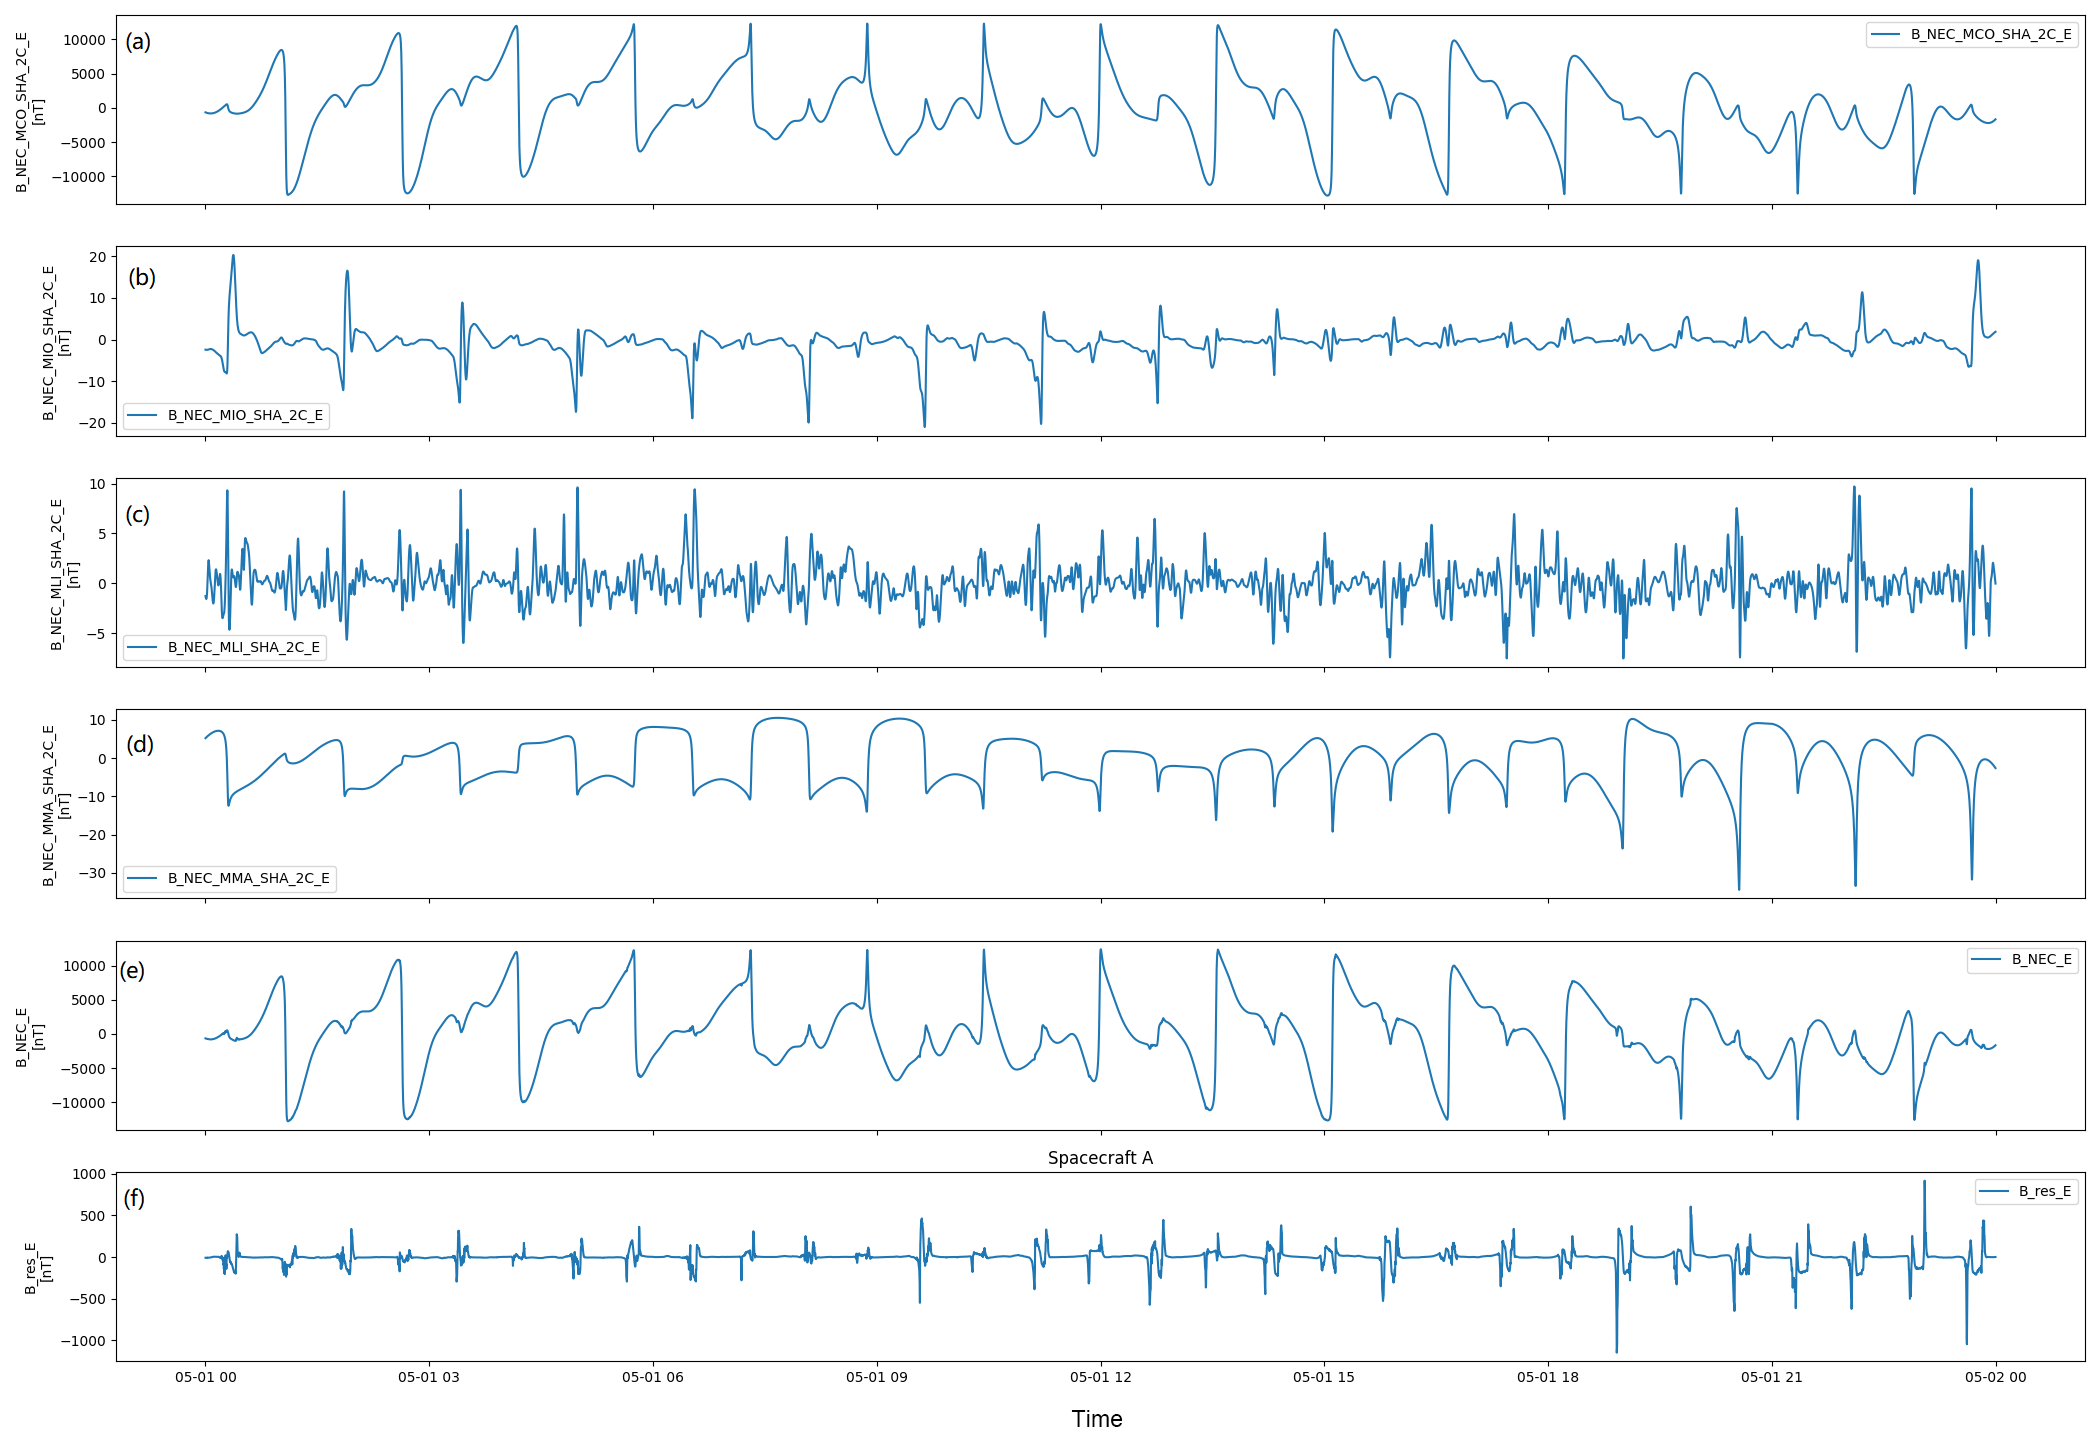
\includegraphics[width=1\linewidth]{CYI4Eng.png}
	\caption{Data of CIY4 model. \hl{Each sub-figure represents the electromagnetic E component data and the electromagnetic E component residual graph, where (a) is the main magnetic field component data, (b) is the ionosphere magnetosphere component data, (c) is the lithosphere magnetic field component data, (d) is the magnetosphere magnetic field component data, (e) is the original observation data, and (f) is the residual of the observation data and the model inversion data.}}
	\label{fig:cyi4}
\end{figure}
\iffalse
\subsection{VMD method}

VMD (Variational Mode Decomposition) \citep{dragomiretskiyVariationalModeDecomposition2014} is a signal decomposition method based on variational principles, which can decompose any signal into a set of oscillatory modes and corresponding auxiliary signals. Unlike traditional signal decomposition methods such as wavelet decomposition and Fourier analysis, VMD does not assume the signal to be stationary or periodic, and it can adaptively extract the local characteristics of the signal. The definition of the mode function $u_k(t)$  is given by Equation \ref{eq:5}, and the analytic signal representation of $u_k(t)$  is expressed in Equation \ref{eq:6}.
\begin{equation}
	\label{eq:5}
	u_k(t)=A_kcos(\varphi_k(t))
\end{equation}

\begin{equation}
	\label{eq:6}
	\begin{array}{l@{\quad}l@{\quad}l}
		Z(t) &= u_k(t) + j\mathscr{H}(u_k(t)) \\
		&= (\delta(t)+\displaystyle{\frac{j}{\pi t})}\ast u_k(t)
	\end{array}
\end{equation}

In Equation \ref{eq:6}, $\mathscr{H}$  denotes the Hilbert transform, and $\delta(t)$  represents the impulse signal. The spectrum is shifted to baseband, as shown in Equation \ref{eq:7}.
\begin{equation}
	\label{eq:7}
	\left[\left(\delta \left(t\right)+\displaystyle{\frac{j}{\pi t}}\right)\ast {u}_{k}\left(t\right)\right]{e}^{-jw_kt}
\end{equation}
The VMD constrained variational model is constructed as shown in Equation \ref{eq:8}. This model aims to minimize the sum of the center frequency bandwidths of each mode under the constraint that the sum of all modes (${\displaystyle \sum\limits_{k} u_k}$ ) equals the given signal $f$ . Solving this variational problem yields the desired decomposition mode functions.
\begin{equation} 
	\label{eq:8}
	\left\lbrace
	\begin{aligned}
		\min_{{u_k,w_k}} \quad \sum_k \left\Vert \partial_t \left[\left(\delta(t) + \frac{j}{\pi t}\right) \ast u_k(t) \right] e^{-jw_kt} \right\Vert_2^2 \\
		\text{s.t.} \quad \sum_k u_k = f
	\end{aligned}\right.
\end{equation}

To solve the variational model's minimum value, an augmented Lagrangian function is constructed by introducing Lagrange multipliers $\lambda$ and penalty factors $\alpha$, as shown in Equation \ref{eq:9}.
\begin{equation}
	\label{eq:9}
	\begin{aligned}
		\mathscr{L}(u_k,w_k,\lambda) = &\alpha \sum_k \left\Vert \partial_t \left[\left(\delta(t) + \frac{j}{\pi t}\right) \ast u_k(t) \right] e^{-jw_kt} \right\Vert_2^2 \\
		&+ \left\Vert f(t) - \sum_k u_k \right\Vert_2^2 + \lambda \langle  f(t) - \sum_k u_k  \rangle
	\end{aligned}
\end{equation}

To solve the extremum problem of the augmented Lagrangian function in a multi-dimensional setting, the Alternating Direction Method of Multipliers (ADMM) \citep{BoydDistributedOptimizationStatistical2011} can be employed. This method iteratively solves the problem by alternately updating each variable while fixing the others. Specifically, each iteration consists of three steps: updating the primal variables, updating the Lagrange multipliers, and projecting onto the constraint set. By repeating these steps, the ADMM algorithm gradually approaches the minimum or maximum of the augmented Lagrangian function. The advantage of using the ADMM algorithm to solve optimization problems is its potential for parallel processing, fast convergence speed, and good stability.
\begin{equation}
	\label{eq:10}
	\begin{aligned}
		u_k^{n+1} &= \operatorname*{argmin}_{{u_k}} \mathscr{L}\left( u_{i<k}^{n+1},w_k^n,\lambda^n \right) \\
		w_k^{n+1} &= \operatorname*{argmin}_{{w_k}} \mathscr{L}\left( u_{ k}^{n },w_{i<k}^{n+1},\lambda^n \right)\\
		\lambda^{n+1} &= \lambda^n + \rho \left( f(t) - \sum_k u_k^{n+1}(t) \right)
	\end{aligned}
\end{equation}

In Equation \ref{eq:10}, $u_k^{n+1}$  is updated by minimizing the augmented Lagrangian function with respect to  $u_k$ . Similarly, $w_k^{n+1}$  is updated by minimizing the function with respect to $w_k$ . $\lambda^{n+1}$  is updated by adding the scaled difference between $f(t)$  and $\sum_k u_k^{n+1}(t)$  to the current Lagrange multiplier $ \lambda^n $  . The parameter $\rho$  controls the step size of the Lagrange multiplier update.

These steps are repeated until convergence is achieved. The resulting $u_k(t)$  and $w_k(t)$ represent the decomposed modes and auxiliary signals, respectively, obtained through the VMD algorithm.
\fi
\subsection{PSO-VMD method}

VMD (Variational Mode Decomposition) \citep{dragomiretskiyVariationalModeDecomposition2014} is a signal decomposition method based on variational principles, which can decompose any signal into a set of oscillatory modes and corresponding auxiliary signals. Unlike traditional signal decomposition methods such as wavelet decomposition and Fourier analysis, VMD does not assume the signal to be stationary or periodic, and it can adaptively extract the local characteristics of the signal.

However, before using the VMD algorithm, it is necessary to determine the penalty coefficient $\alpha$  and the number of modes $K$  in advance. The selection of these two parameters directly affects the results of the VMD algorithm. If $K$  is too large, it may lead to over-decomposition, while if it is too small, it may result in under-decomposition. The value of $\alpha$  affects the bandwidth of each mode. A smaller $\alpha$  leads to larger bandwidth for each mode, which may cause overlapping passbands among the modes. On the other hand, a larger $\alpha$  leads to smaller bandwidth, which may result in the loss of signal information. Therefore, to determine appropriate values for $\alpha$  and $K$ , this study adopts the Particle Swarm Optimization (PSO)-based VMD algorithm (referred to as PSO-VMD hereinafter). By using the PSO algorithm to adaptively search for the optimal $\alpha$  and $K$  values, the subjectivity and limitations associated with manual parameter selection can be avoided.

The Particle Swarm Optimization (PSO) algorithm treats each solution as a particle in the entire solution space. Each particle is initialized with its initial position and velocity, and it moves in the solution space at a unit time according to the direction and step size determined by its own best local history and the best history of the collective particles. By starting from random positions in the solution space, multiple particles avoid the drawback of a single particle getting trapped in local optima. Compared to other optimization algorithms, PSO algorithm has advantages such as strong global search capability, easy implementation, fast convergence speed, etc., making it suitable for solving complex optimization problems. The update equations for the particle velocity and position are shown in Equation \ref{eq:11}.
\begin{equation}
	\label{eq:11}
	\begin{split}
		& v_{i}^{t+1} = w v_{i}^t + c_1 r_1 (pbest_{i} - x_{i}^t) + c_2 r_2 (gbest - x_{i}^t) \\
		& x_{i}^{t+1} = x_i^t + v_i^{t+1}
	\end{split}
\end{equation}

In the PSO-based VMD algorithm, $v_{i}^t$  represents the velocity of particle $i$  at the  $t-th$ iteration, and $x_i^t$  represents the position of particle $i$  at the  $t-th$ iteration. $pbest_{i}$  denotes the best position (local optimum) achieved by particle  $i$ throughout its history, and $gbest$  represents the best position (global optimum) obtained by any particle in the swarm. $r_1$ and $r_2$  are random numbers between 0 and 1, used to introduce randomness to the particles' movements and prevent them from being trapped in local optima.

The remaining three coefficients in the algorithm, $w$ , $c_1$  and $c_2$ , represent the inertia weight, cognitive weight, and social weight, respectively. The inertia weight   determines the influence of a particle's previous velocity on its current velocity. A higher value of $w$  means that the particle's direction of iteration is less likely to change. The cognitive weight $c_1$  controls the particle's tendency to move towards its personal best position, while the social weight  $c_2$ determines the degree of influence from the swarm's global best position.

In the context of the VMD algorithm, $K$  and $\alpha$  are treated as the position parameters of the particles. The loss error is calculated as the residual of the sum of all modes, as shown in Equation \ref{eq:12}. The  $L^2$ norm, denoted by $\left\Vert\cdot\right\Vert_2$ , is used to measure the magnitude of the residual.
\begin{equation}
	\label{eq:12}
	\displaystyle
	u_{error} = \left\Vert f(t)- \sum_k u_k(t) \right\Vert_2
\end{equation}

The inputs are the electromagnetic data $f(t)$  and the number of iterations $Iter$, and the output is the decomposed modal data $u_k$. In the algorithm, the particle swarm is constructed by setting the number of particles $num$  and initializing their initial states. The parameters for the PSO algorithm are also set. In each iteration, the VMD decomposition $u_k^j$  is computed for the current particle state (as shown in Equation \ref{eq:10}). The particle states are updated by calculating the residual (as shown in Equation \ref{eq:12}) and recording the individual best solution $pbest_{i}$  as well as the global best solution $gbest$  (as shown in Equation \ref{eq:11}). After each particle completes one iteration, the next iteration begins. Once all iterations are completed, the VMD decomposition values are computed based on $gbest$, and the modal data $u_k$  is returned.

After completing all iterations, the VMD decomposition values are obtained based on the global best position $gbest$ . The modal data $u_k$  can then be extracted from the VMD decomposition.

Algorithm \ref{al:PSO-based-VMD} delineates the complete procedural flow of PSO-based Variational Mode Decomposition (VMD). This algorithm takes electromagnetic data $f(t)$ and the number of iterations $Iter$ as inputs and yields the decomposed mode data $u_k$ as output. The algorithm {which is listed below} begins by constructing the particle swarm through initializing the number of particles as $num$ and specifying their initial states. Additionally, the iteration coefficient for the particle swarm algorithm is set. Within each iteration, the VMD decomposition $u_k^j$ is computed under the current state of each particle (refer to Equation \ref{eq:10}). The state of each point is updated by evaluating the residual (as shown in Equation \ref{eq:12}), while simultaneously recording the individual best solution $pbest_j$ and the global best solution $gbest$ (as depicted in Equation \ref{eq:11}). Once all particles have completed one iteration, the algorithm proceeds to the next iteration. Upon completion of all iterations, the VMD decomposition value is computed based on $gbest$, and the resulting solution $u_k$ is returned. 
\begin{algorithm}[htb]
	\renewcommand{\algorithmicrequire}{\textbf{input:}}
	\renewcommand{\algorithmicensure}{\textbf{output:}}
	\caption{PSO-based-VMD}
	\label{al:PSO-based-VMD}
	\begin{algorithmic}[1]
	\REQUIRE  electromagnetic$f(t)$and the number of iterations{ }$Iter$  
	\ENSURE the decomposed mode data{ }$u_k$ 	
	\STATE initializing the number of the particles{ }$num$ and specifying their initial states;
	\FOR {$i=1,2,\cdots,Iter$}
		\FOR {$j=1,2,\cdots,num$}
			\STATE Perform VMD decomposition $u_k^j$ based on the current particle state
			\STATE Update the state of each point using the residual calculation
			\STATE Update the individual best solution $pbest_j$ and the global best solution $gbest$
		\ENDFOR
	\ENDFOR	
	\STATE Calculate the VMD decomposition value based on $gbest$
		
	\STATE \textbf{return} $u_k$;
	\end{algorithmic}
\end{algorithm}

The PSO-based VMD algorithm offers several advantages. First, it automatically determines the optimal values of the parameters {$K$}  and $\alpha$  through the particle swarm optimization process, eliminating the subjective and limited manual selection. Second, the PSO algorithm's global search capability helps {to avoid getting trapped} in local optima, leading to better decomposition results. Third, the PSO algorithm is computationally efficient and can handle complex optimization problems.

Overall, the PSO-based VMD algorithm provides an effective and automatic approach for decomposing signals into modal components and auxiliary signals. By adaptively determining the values of $K$  and {$\alpha$} , it ensures accurate and reliable signal decomposition, enabling the extraction of meaningful features and improving the analysis of the original signals.
\subsection{ECOD method}
ECOD (Empirical Cumulative Outlier Detection) is an unsupervised outlier detection method that effectively detects outliers in data \citep{LiECODUnsupervisedOutlier2022}. This method is based on the Empirical Cumulative Distribution Function (ECDF), which is a non-parametric empirical distribution function representing the proportion of data points in a dataset that are less than or equal to a given value. To ensure outlier detection in different directions, ECOD calculates the left-tail ECDF and right-tail ECDF of the data in the  $j-th$ dimension, as shown in Equation \ref{eq:13}. Here, $x_i^j$ represents the  $j-th$ dimensional value of the  $i-th$ sample, $n$  is the total number of samples, and $1(\cdot)$  is the indicator function. $F_{left}^j(z)$  represents the proportion of samples in the  $j-th$ dimension that are less than or equal to $z$, i.e., the left-tail ECDF, while  $F_{right}^j(z)$  represents the proportion of samples in the  $j-th$ dimension that are greater than or equal to $z$, i.e., the right-tail ECDF. By calculating the left-tail ECDF and right-tail ECDF in each dimension, ECOD constructs a multi-dimensional ECDF in the multi-dimensional space and utilizes it for outlier detection of multi-dimensional data.
\begin{equation}
	\label{eq:13}
	\begin{split}
		&F_{left}^j(z) =  \frac{1}{n}\sum_{i=1}^{n} 1(x_i^j \leq z) \\
		&F_{right}^j(z) =  \frac{1}{n}\sum_{i=1}^{n} 1(x_i^j \geq z) 
	\end{split}
\end{equation}

To calculate the skewness of the data in the  $j-th$ dimension, this paper uses the sample's third central moment as a measure of skewness, as shown in Equation \ref{eq:14}. This skewness value will serve as a reference for the final outlier score. Here, $\operatorname{SK}$  represents the skewness, $E\left[\cdot \right]$ denotes the mathematical expectation, $X$ represents a random variable,  $\mu$ represents the mean, $\sigma$  represents the standard deviation, $x_i$  represents the  $i-th$ sample,  $\bar{x}$ represents the sample mean, and {$n$} represents the sample size.
\begin{equation}
	\label{eq:14}
	\begin{split}
		\operatorname{SK}
		& = E\left[ \left( \frac{X-\mu}{\sigma}\right)^3 \right]  \\
		&= \frac{\frac{1}{n} \sum_{i=1}^{n} (x_i - \bar{x})^3}{\left(\frac{1}{n} \sum_{i=1}^{n} (x_i - \bar{x})^2\right)^{\frac{3}{2}}}
	\end{split}
\end{equation} 

In ECOD, there are three components involved in calculating the outlier scores: left-only value, right-only value, and auto value $O_{auto}(X_i)$, as shown in Equation \ref{eq:15}.
\begin{equation}
	\label{eq:15}
	\begin{split}
		O_{left\_only}(X_i) &= - \sum_{j=1}^{d} \log \left( F_{left}^j\left( X_i^j \right) \right) \\
		O_{right\_only}(X_i) &= - \sum_{j=1}^{d} \log \left( F_{right}^j \left( X_i^j \right) \right) \\
		O_{auto}(X_i) &= - \sum_{j=1}^{d} [ 1\{ SK_j < 0 \}\log (F_{left}^j(X_i^j)) \\ & \quad \quad + 1\{ SK_j >= 0 \}\log (F_{right}^j(X_i^j))]  
	\end{split}
\end{equation}

In outlier detection, the larger the value of $O(\cdot)$, the farther the data point is from the collective characteristics of the entire dataset, indicating a higher likelihood of being an outlier. $O_{left\_only}(X_i)$ represents the distance of data point $X_i$  from the left-tail outliers, while $O_{right\_only}(X_i)$  represents the distance from the right-tail outliers. $O_{auto}(X_i)$ considers the skewness of each feature in $X_i$  to determine which direction of outliers to consider. 

Specifically, if the skewness of the  $j-th$ feature is less than 0, indicating a right-skewed distribution, the left-tail outliers are more likely, so the left-tail outliers are used. Conversely, if the skewness of the  $j-th$ feature is greater than or equal to 0, indicating a left-skewed distribution, the right-tail outliers are more likely, so the right-tail outliers are used. The maximum value among $O_{left\_only}(X_i)$ , $O_{right\_only}(X_i)$ , and $O_{auto}(X_i)$  is taken as the outlier score $O_i$  for data point $X_i$ , as shown in Equation \ref{eq:16}.
\begin{equation}
	\label{eq:16}
	O_i = \max \left\lbrace   O_{left\_only}(X_i),	O_{right\_only}(X_i),	O_{auto}(X_i)   \right\rbrace 
\end{equation}

This outlier score $O_i$  helps identify the extent to which a data point deviates from the overall distribution of the dataset, thereby indicating its likelihood of being an outlier.   
\section{Results and Discussion}

{In order to verify the effectiveness of the anomaly detection method proposed in this study, this study selected an incident that occurred on September 15, 2016, 11 kilometers north-northeast of La Paz Centro urban area in Leon Province, Nicaragua (west longitude $86^\circ$, north latitude $12^\circ$) of a shallow earthquake of magnitude 5.7. After obtaining electromagnetic data from the swarm satellite in the time range from 6 months before the earthquake to 3 months after the earthquake, anomalies were detected within this interval. After obtaining the electromagnetic data, effective earthquake-related signals are obtained by removing the static field and dynamic field of the earth. On this basis, the data is segmented. The segmentation is based on the orbit number (OrbitNumber) of the Swarm satellite. For the Swarm A satellite, it is in a near-polar orbit with an altitude of 462-524 kilometers and an orbital inclination of 87.4 degrees. run. In this orbit, the Swarm A satellite takes approximately 91 minutes to orbit the Earth. Therefore, the data time span of each piece of data is 91 minutes.}

Figure \ref{fig:nicaragua} presents {the geographic distribution of earthquake epicenters} with a magnitude greater than 5.0 in the Nicaragua region from 2000 to the present (March 4, 2023). In the {Figure}, the size of the blue dots represents the magnitude intensity of each earthquake. Furthermore, the red {star} in the figure indicates the location of {the seismic event selected in this survey}.
\begin{figure}[htbp]
	\centering
	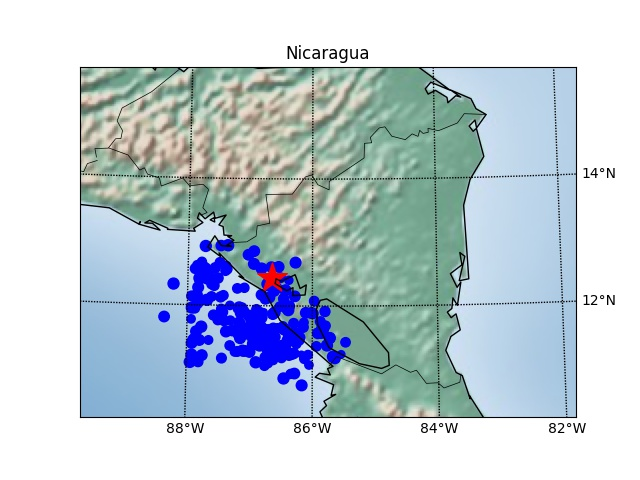
\includegraphics[width=0.8\linewidth]{Nicaragua_1990-01-01-2024-01-01}
	\caption{\hl{Nicaragua earthquake distribution map. Each point in the map represents the location of an earthquake with a magnitude greater than 5. The size of the blue point represents the magnitude intensity, and the red asterisk represents the earthquake selected in the experiment.}}
	\label{fig:nicaragua}
\end{figure}

As shown in Figure \ref{fig:pre-earthquake-anomaly-detection-Nicaragua}, Figure \ref{fig:raw-data-anomaly-detection-Nicaragua} displays the cumulative results obtained by applying the ECOD method directly to {the original data} without utilizing the PSO-VMD method for preprocessing. On the other hand, Figure \ref{fig:PSO-VMD-anomaly-detection-Nicaragua} represents the cumulative results obtained after applying the PSO-VMD method for preprocessing. Since the trend of the {sigmoid function}\citep{oksumNovelApproachBased2021} is gradual-steep-gradual, fitting the cumulative results with the sigmoid function allows for a better representation of the pre-earthquake anomaly trend. Consequently, the fitted Sigmoid function is utilized to discern the trend of the critical anomaly.
\begin{figure}[htbp]
	\centering
	\subfloat[Anomaly detection based on raw data]{
		\label{fig:raw-data-anomaly-detection-Nicaragua}
		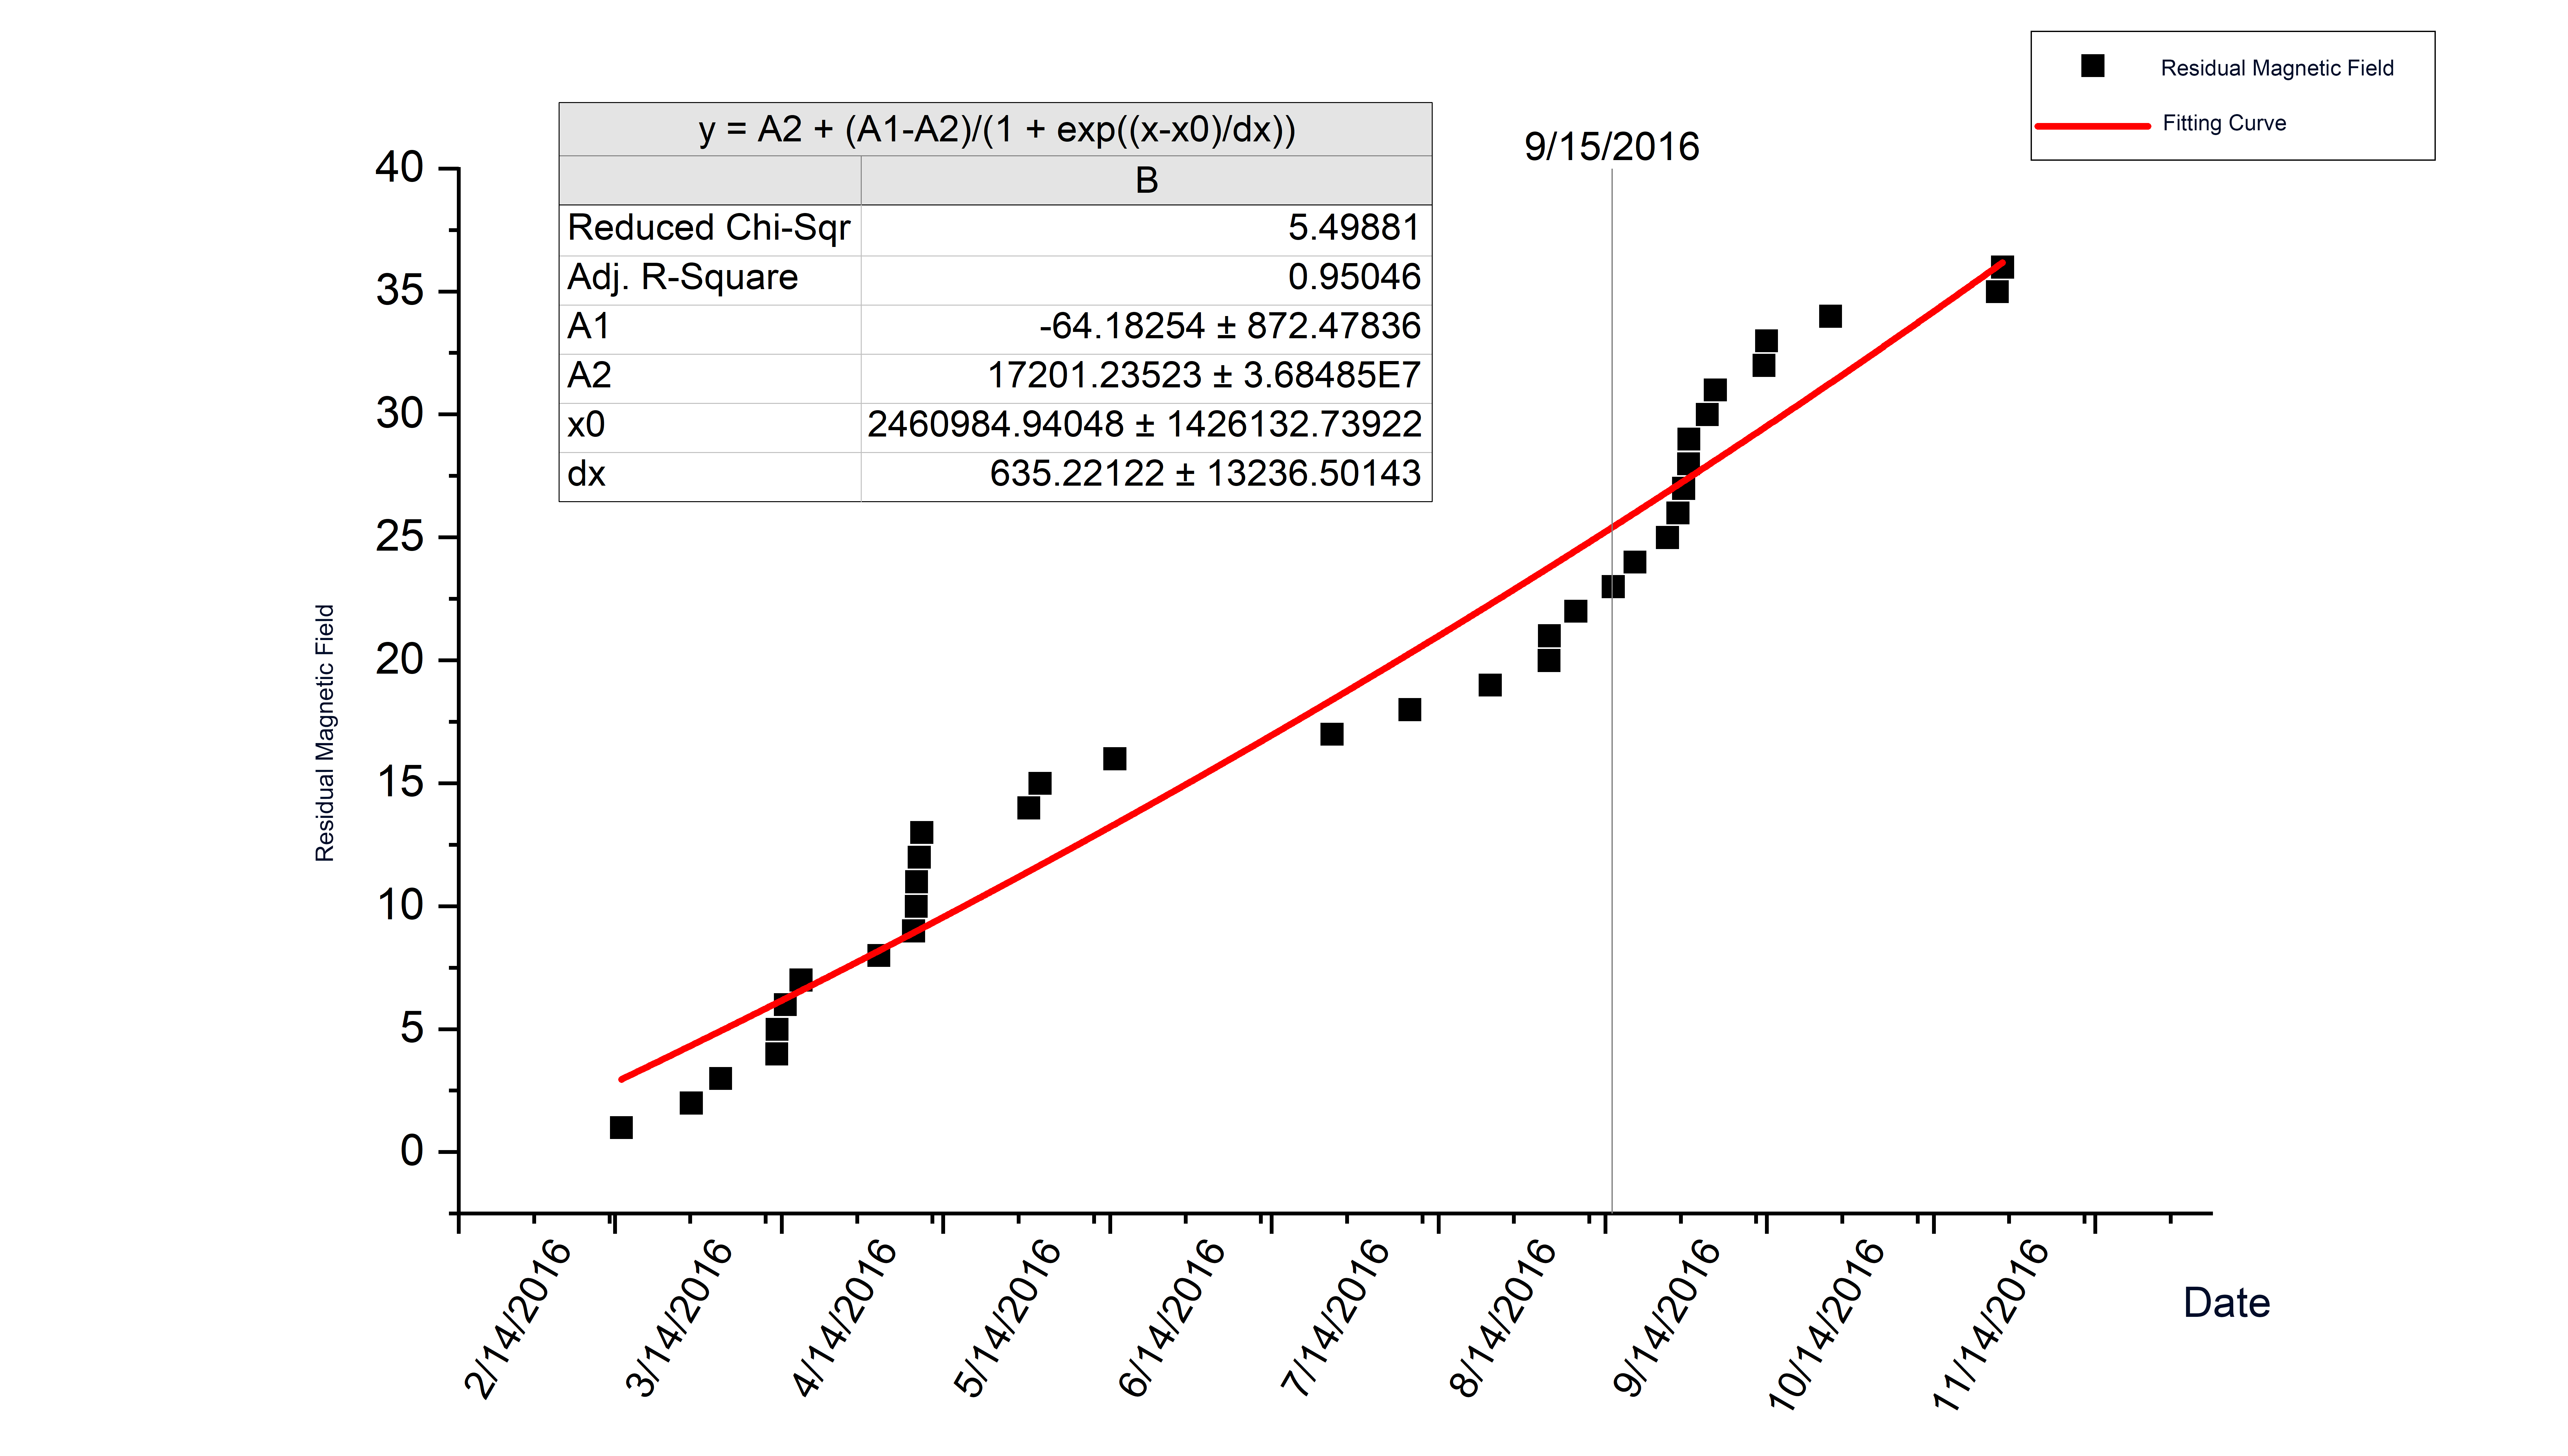
\includegraphics[width=.45\linewidth]{Nicaragua_rawEng.png}}
	\subfloat[Anomaly detection based on PSO-VMD]{
		\label{fig:PSO-VMD-anomaly-detection-Nicaragua}
		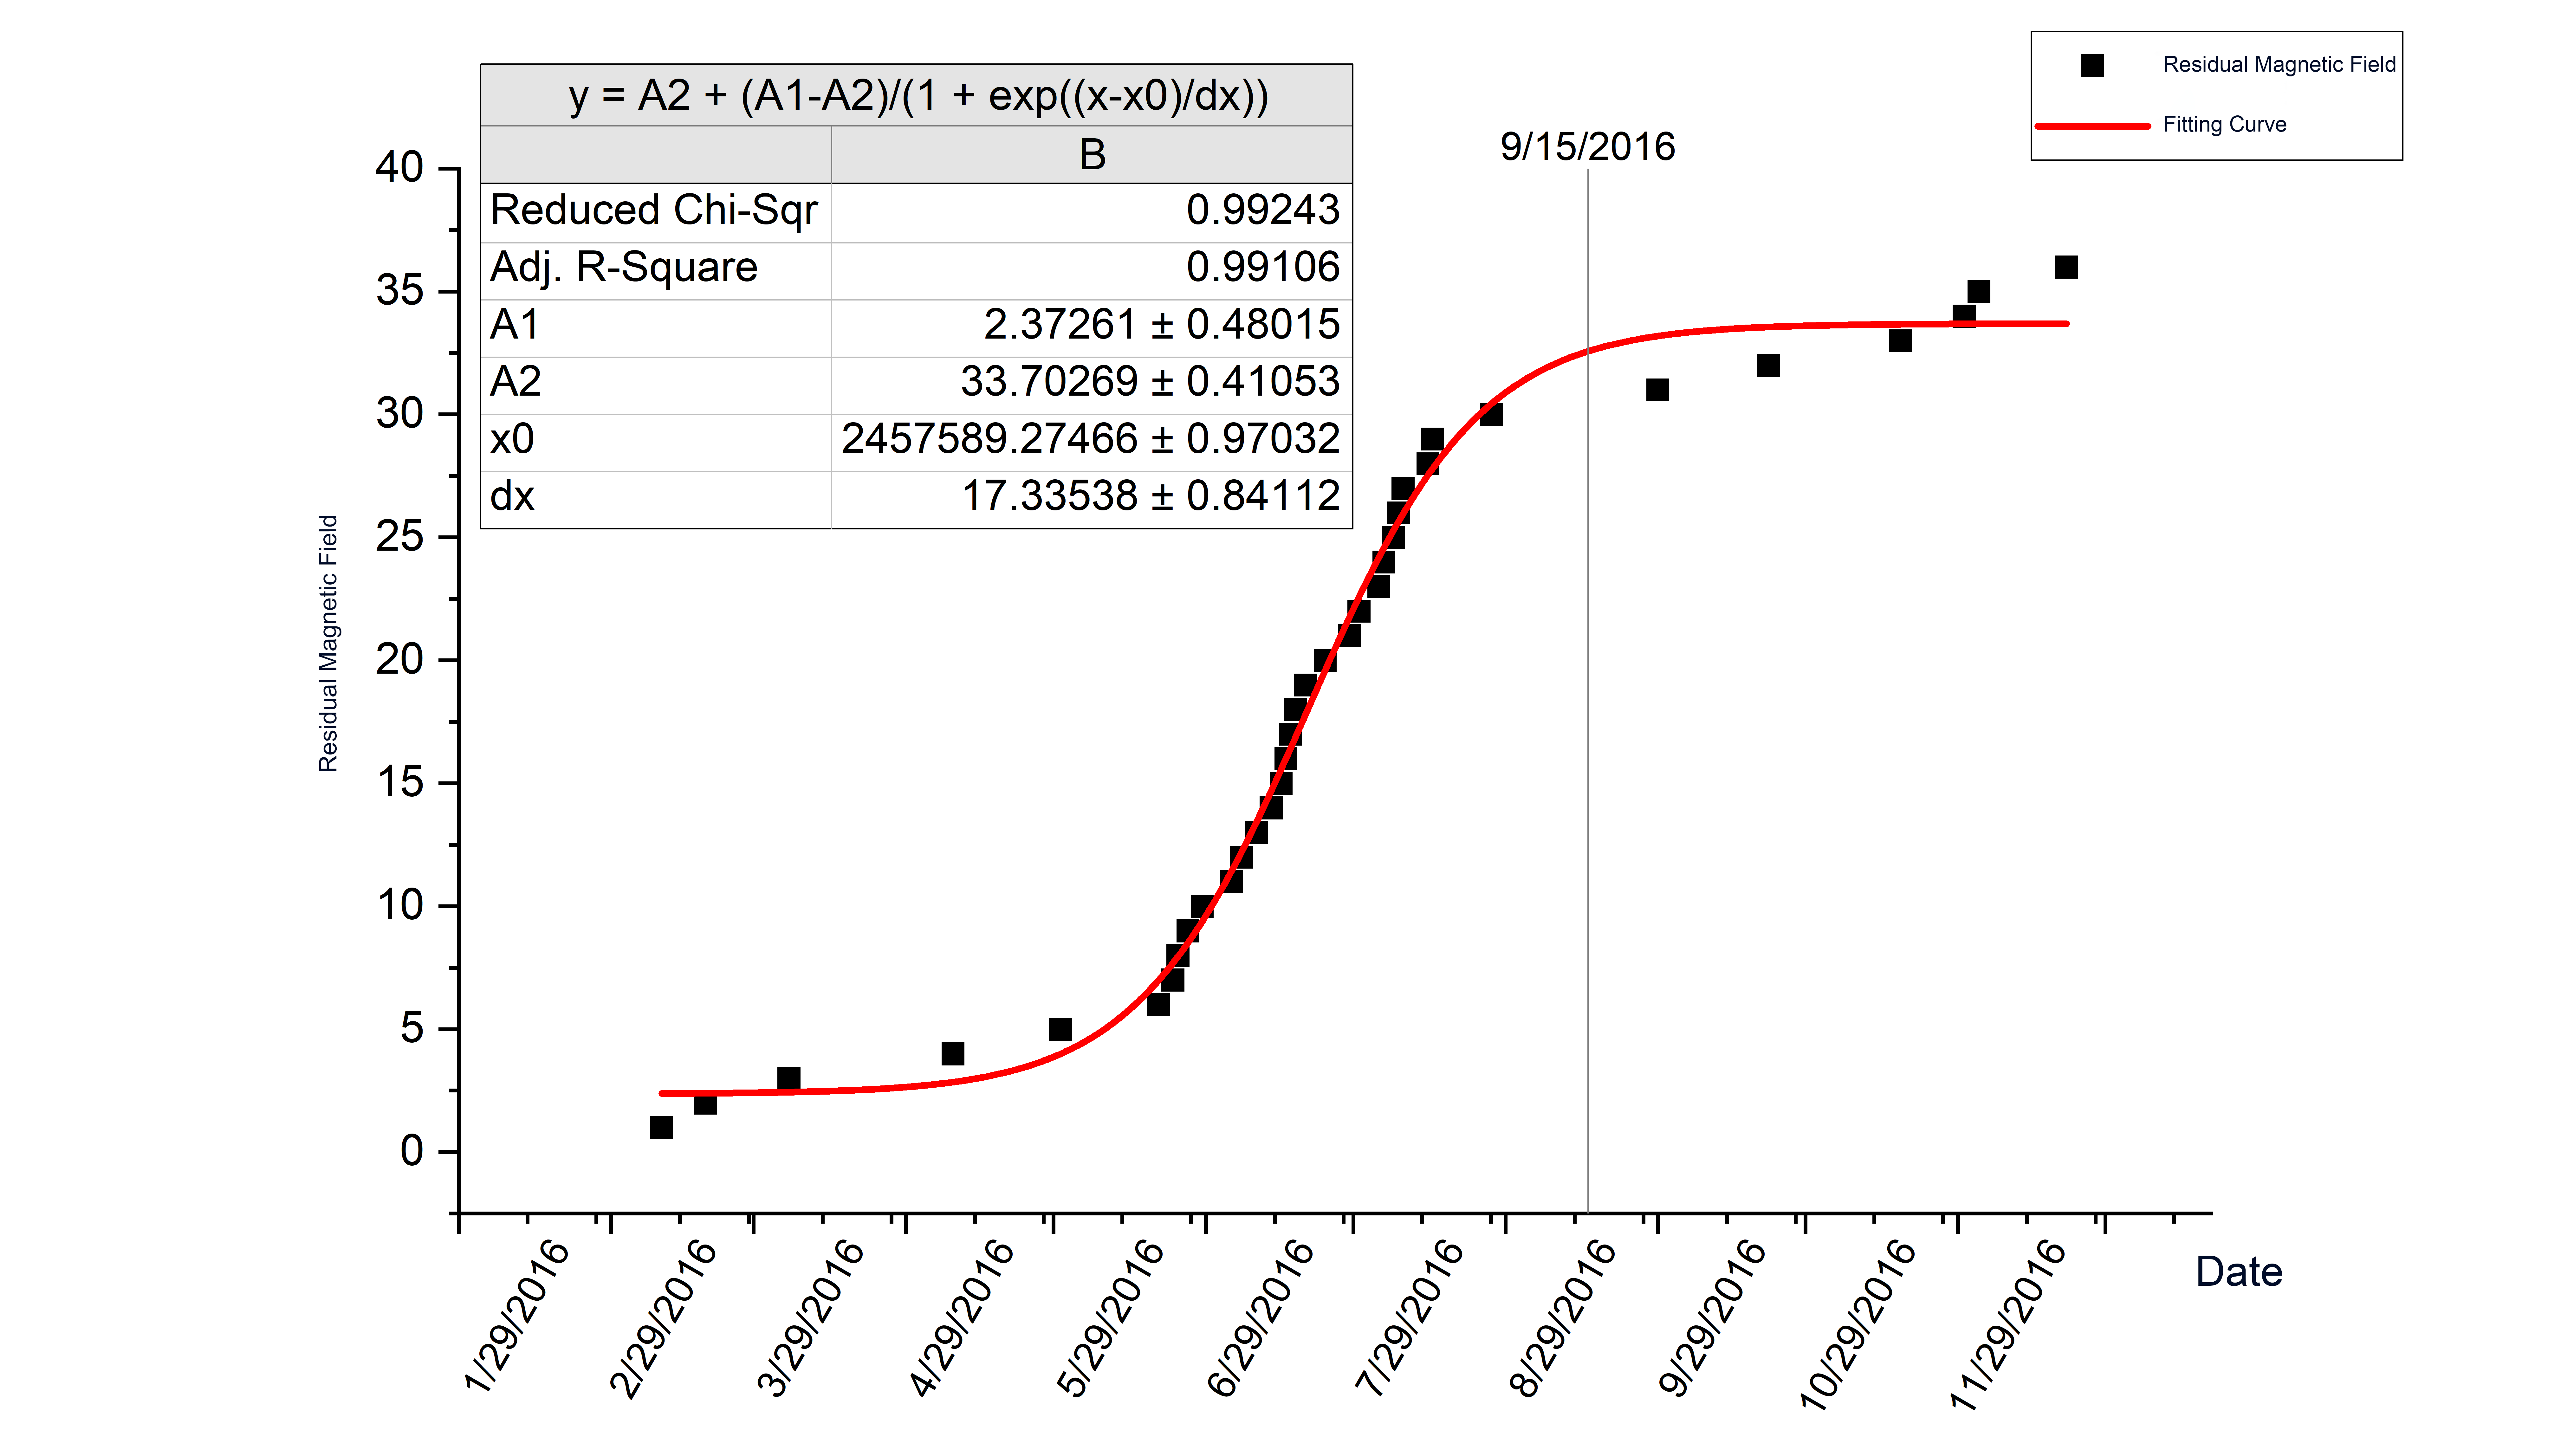
\includegraphics[width=.45\linewidth]{Nicaragua_VMDEng.png}}
	\caption{{Pre-earthquake anomaly detection comparision of Nicaragua between raw data and preprocessed data with PSO-VMD.}}
	\label{fig:pre-earthquake-anomaly-detection-Nicaragua}
\end{figure}

To determine whether anomalies are related to earthquakes, analysis can be conducted by calculating cumulative anomalies. If the cumulative anomalies show a linear increasing trend, it indicates a random process. Conversely, if the cumulative anomalies exhibit a sharp rise before the earthquake, especially with multiple sudden anomalies occurring in the period leading up to the earthquake, followed by a return to stability after the earthquake, it can be concluded that there is a strong correlation between the anomalies and the earthquake event. Since the trend of {the sigmoid function} (Equation \ref{eq:17}) is gradual-steep-gradual, fitting the cumulative results with a sigmoid function can better characterize the trend of pre-earthquake anomalies, allowing the identification of critical anomaly trends. {Compared with other sigmoid functions (such as Logistic function, Hill function, SWeibull function), the Boltzmann function has more adjustment parameters, so this study chose it as the fitting function.} The adjusted sigmoid function is Boltzmann function like Equation \ref{eq:17}, {where $A_1$ controls the upper bound of the function, and the $A_2$ control the lower bound, $x_0$ controls the growth inflection point, and $dx$ controls the growth slope.} 
\begin{equation}
	\label{eq:17}
	f(x) = A_2 + \frac{A_1-A_2}{1+e^{-\frac{(x-x_0)}{dx}}}
\end{equation}

To provide an initial assessment of the fitting results, this study utilizes the Adjusted R-Squared coefficient. The main purpose of Adjusted R-Squared is to measure the difference between the fitting results and the original data. Equation \ref{eq:18} represents the calculation method of Adjusted R-Squared, where RSS denotes the residual sum of squares of the regression model, TSS represents the total sum of squares of the data, {$n$ is the sample size and $p$ is the number of independent variables}. Compared to R-Squared, Adjusted R-Squared adjusts R-Squared based on the sample size and the number of independent variables to account for the influence of irrelevant dimensions on the fitting results. {The use of Adjusted R-Square in this study can better reflect the correlation between the abnormal accumulation trend and the fitting function, so as to better study pre-earthquake anomalies.}

\begin{equation}
	\label{eq:18}
	\left\lbrace\begin{split}
		& R^2 = 1 - \frac{RSS}{TSS} = 1 - \frac{\sum \left(  y - \hat{y} \right)^2}{\sum \left( y - \bar{y} \right)^2} \\
		& R_{adj}^2 = 1 -  \frac{\left(1-R^2\right)\left(n-1\right)}{n-p-1} 
	\end{split}\right.
\end{equation}

{In order to further study the generalization ability of this method, we randomly selected multiple earthquake events and non-earthquake events and applied this method to perform pre-earthquake anomaly detection.} {Within the year 2016, a random selection of events was made.} The time range for the selected events was 180 days before and 90 days after the given earthquake occurrences. Among the selected events, there were a total of 6 earthquake events and 14 non-earthquake events (no earthquakes greater than magnitude 5 occurred within the given grid). The detailed information of the earthquake and non-earthquake events is presented in Tables \ref{tab:random earthquake event} and Tables \ref{tab:random non earthquake event}, respectively.
\begin{table}[htbp]
	\caption{random earthquake event}
	\label{tab:random earthquake event}
	\centering
	\begin{tabular}{clccc}
		\toprule
		\textbf{Index} & \textbf{Date} &\textbf{Latitude}&\textbf{Longitude}&\textbf{Magnitude Level} \\
		\midrule
		\textbf{A}&2016/3/18 16:11 & 43$^\circ$     & 72$^\circ$     & 5.6  \\
		\textbf{B}&2016/4/2 5:50   & 62$^\circ$     & -155$^\circ$   & 5.9  \\
		\textbf{C}&2016/3/10 3:24  & -55$^\circ$    & -66$^\circ$    & 5.2  \\
		\textbf{D}&2016/5/28 9:46  & -57.74$^\circ$ & -27.15$^\circ$ & 7.2 \\
		\textbf{E}&2016/9/15 5:57  & 13$^\circ$     & -85.75$^\circ$ & 5.7 \\
		\textbf{F}&2016/5/28 4:43  & 5$^\circ$      & -38$^\circ$    & 5.2 \\
		\bottomrule
	\end{tabular}
\end{table}
\begin{table}[htbp]
	\caption{random non earthquake event}
	\label{tab:random non earthquake event}
	\centering
	\begin{tabular}{clcc|clcc}
		\toprule
		\textbf{Index}&\textbf{Date}               & \textbf{Lat}  & \textbf{Lon}  &\textbf{Index}&\textbf{Date}               & \textbf{Lat}  & \textbf{Lon}  \\ \midrule
		\textbf{A}&2016/5/27 19:32 & -71$^\circ$ & -60$^\circ$  &\textbf{H} &2016/8/22 16:41  & -24$^\circ$ & -49$^\circ$ \\
		\textbf{B}&2016/8/13 2:18  & 54$^\circ$  & 89$^\circ$   &\textbf{I}& 2016/8/21 17:40 & -15$^\circ$ & 146$^\circ$ \\
		\textbf{C}&2016/5/6 20:24   & -45$^\circ$ &115$^\circ$ & \textbf{J}&2016/6/12 10:49  & 38$^\circ$  & 11$^\circ$  \\
		\textbf{D}&2016/4/10 21:59  & 36$^\circ$  & -103$^\circ$ &\textbf{K} &2016/7/25 3:31   & 34$^\circ$  & 114$^\circ$ \\
		\textbf{E}&2016/8/26 6:32   & 67$^\circ$  & -173$^\circ$ & \textbf{L}&2016/8/21 1:22   & -63$^\circ$ & -71$^\circ$ \\
		\textbf{F}&2016/6/8 20:35   & -35$^\circ$ &15$^\circ$ & \textbf{M}&2016/5/20 9:51   & 68$^\circ$  & 138$^\circ$ \\
		\textbf{G}&2016/6/9 21:50  & 65$^\circ$  & 46$^\circ$   &\textbf{N}& 2016/4/21 14:11  & 18$^\circ$  & 69$^\circ$  \\ \bottomrule
	\end{tabular}
\end{table}

The earthquake events and non-earthquake events have undergone data preprocessing, signal classification, and anomaly detection, and the results have been fitted. Figure \ref{fig:random earthquake event analysis} shows the final results. The time scale for all events is constrained between -180 days and 90 days. In the figure, the gray line represents the occurrence of earthquake events.
\begin{figure}[htbp]
	\centering
	\subfloat[Earthquake event anomaly detection]{
		\label{fig:earthquake event anomaly detection}
		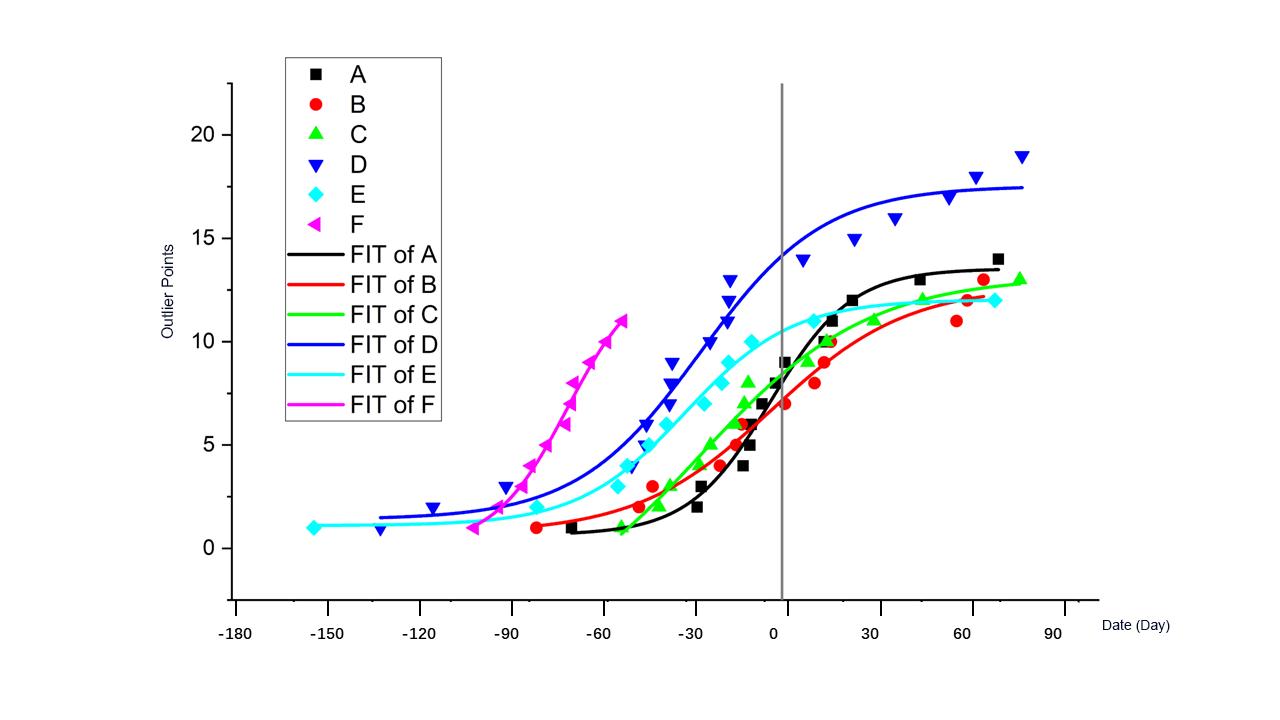
\includegraphics[width=0.8\linewidth]{TRUE_FITEng}} \\
	\subfloat[Non-seismic events (part 1)]{
		\label{fig:non-seismic events (part 1)}
		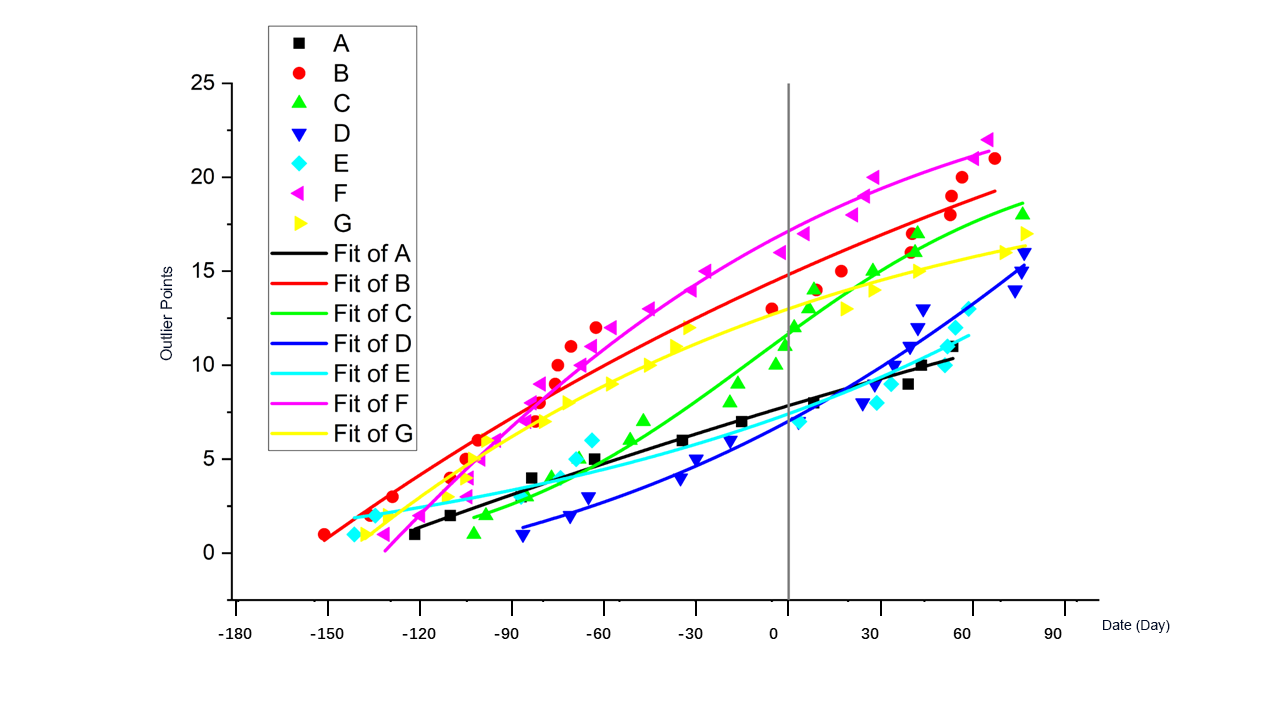
\includegraphics[width=0.49\linewidth]{FALSE_FIT1Eng}}
	\subfloat[Non-seismic events (part 2)]{
		\label{fig:non-seismic events (part 2)}
		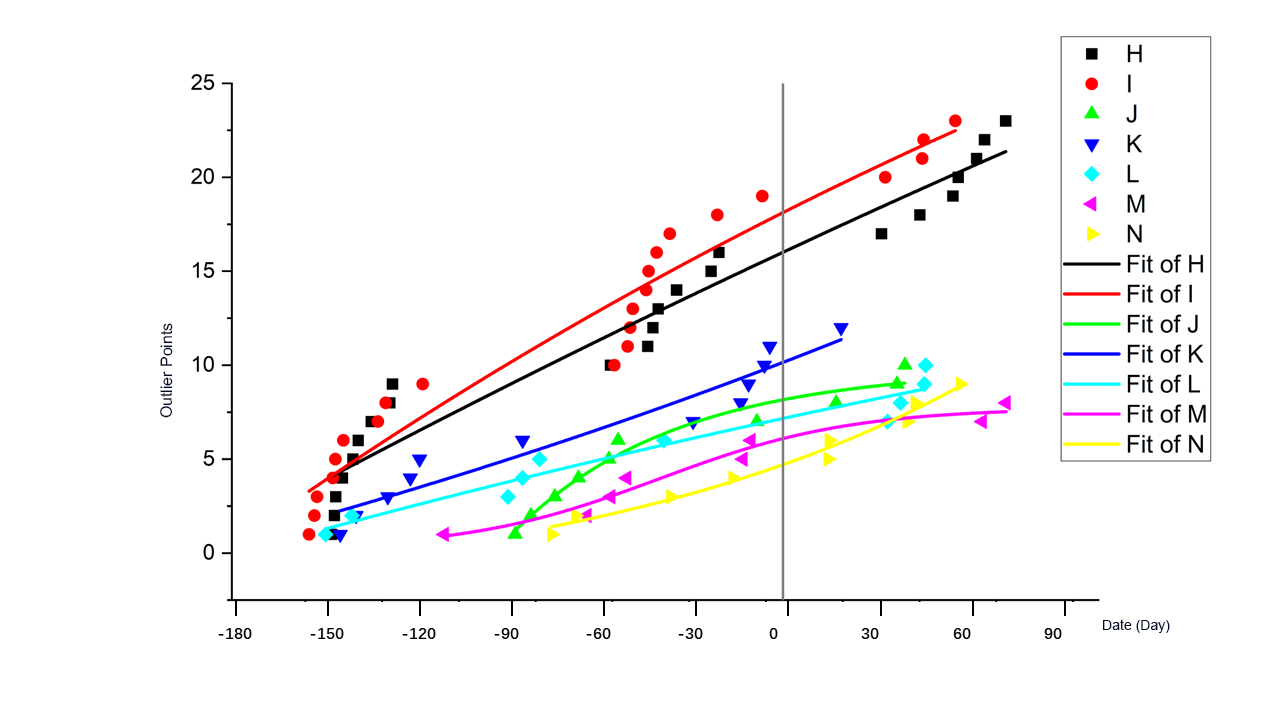
\includegraphics[width=0.49\linewidth]{FALSE_FIT2Eng}}
	\caption{Random earthquake event analysis}
	\label{fig:random earthquake event analysis}
\end{figure}

Figure \ref{fig:earthquake event anomaly detection} represents the results of anomaly detection for earthquake events. It is evident that there is a significant increase in the number of outlier points at the occurrence of earthquake events. Furthermore, these outlier points follow the trend of a Sigmoid function more closely. In contrast, the data during non-earthquake events, as shown in Figure \ref{fig:non-seismic events (part 1)} and Figure \ref{fig:non-seismic events (part 2)}, exhibit smaller increases in the fitted anomalies, which are closer to linear and thus more consistent with the probability of random event occurrences.

To qualitatively study the fitting quality, we will use the given $R_{adj}^2$  in {Equation} \ref{eq:18} as a criterion to compare the linear fitting and Boltzmann function fitting for earthquake and non-earthquake events. Additionally, we will use the ratio of the Boltzmann function-fitted $R_{adj}^2$  to the linear-fitted $R_{adj}^2$ , as shown in {Equation} \ref{eq:18}, and take its logarithm as a basis. If this ratio is greater than 0, it indicates that the curve is closer to the Boltzmann function; if the ratio is less than 0, it indicates that the curve is closer to a linear function. Furthermore, we will use two parameters to assist in assessing the quality of the fitting results. {$x_0$}, which represents the time difference between the Boltzmann function-fitted center value and the occurrence of earthquake events, will be used to determine if the fitting result detects anomalies within a reasonable time. {The larger the absolute value of $x_0$ is, the greater the difference between the detected anomaly and the earthquake occurrence time is, and the weaker the correlation.} $dx$  will characterize the growth trend of the Boltzmann function and can indicate the magnitude of anomaly amplitudes.
\begin{equation}
	\label{eq:19}
	R_{ratio} = \log(\frac{R_{Boltzmann}^2}{R_{linear}^2}) \times 100
\end{equation}

According to Table 4 and Table 5, $x_0$  represents the number of days relative to the occurrence of the earthquake, where negative values indicate pre-earthquake and positive values indicate post-earthquake. $dx$  represents the rate of anomaly accumulation, and its value is converted to the ratio with the average value of all $dx$  data. The closer the value is to 0, the more pronounced the rate of anomaly accumulation. Regarding earthquake events, we can observe from Table 4 that almost all $x_0$  values are close to the occurrence of the event, and $R_{ratio}$ values are greater than 0, indicating that the trend of outlier points is closer to the Boltzmann function rather than linear growth. Additionally, the {$dx$}  values are close to 0, indicating significant increases in anomaly rates occurring before the earthquake.

{However, for the anomaly detection result indicators} in the non-earthquake time period in Table \ref{tab:Non Earthquake Event Anomaly Detection Result Metrics}, almost all values are unreasonable. For example, events A, E, H, I, J, and L are closer to the fitting result of random events. For events B, G, K, and N, the inflection points are too far from the events, making them meaningless in practical terms. Although the data point M may seem reasonable, it is actually due to a small value of $\vert A_1 - A_2 \vert$ , which is 7. This means that although there is some level of anomaly, the perturbation is small and can be ignored.
\begin{table}[htbp]
	\caption{Earthquake Event Anomaly Detection Result Metrics}
	\label{tab:Earthquake Event Anomaly Detection Result Metrics}
	\centering
	\begin{tabular}{crrr}
		\toprule
		\textbf{Index}& $R_{ratio}$ & $x_0$       & $dx$    \\
		\midrule
		\textbf{A} & 5.08392     & -4     & 0.06 \\
		\textbf{B} & 1.034487    & -4     & 0.10 \\
		\textbf{C} & 3.362188    & -30    & 0.12 \\
		\textbf{D} & 1.896997    & -30    & 0.09 \\
		\textbf{E} & 8.724399    & -36    & 0.08 \\
		\textbf{F} & 0.664581    & -79    & 0.05 \\
		\bottomrule
	\end{tabular}
\end{table}
\begin{table}[htbp]
	\caption{Non Earthquake Event Anomaly Detection Result Metrics}
	\label{tab:Non Earthquake Event Anomaly Detection Result Metrics}
	\centering
	\begin{tabular}{crrr|crrr}
		\toprule
		\textbf{Index}& $R_{ratio}$ & $x_0$ & $dx$   &   \textbf{Index}   & $R_{ratio}$ & $x_0$ &  $dx$   \\
		\midrule
		\textbf{A} & -0.14521    & -2282 & 2.65 & \textbf{H} & -0.25267    & -2873 & 4.58 \\
		\textbf{B} & 0.053099    & -1614 & 1.46 & \textbf{I} & -0.12263    & -1995 & 2.19 \\
		\textbf{C} & 0.105649    & \textbf{-13}   & 0.22 & \textbf{J} & 1.982042    & -537  & 0.25 \\
		\textbf{D} & 0.655548    & 169   & 0.46 & \textbf{K} & -0.94167    & 2728  & 2.32 \\
		\textbf{E} & -0.016      & 1232  & 0.74 & \textbf{L} & -1.04415    & -2358 & 2.83 \\
		\textbf{F} & 1.071618    & -207  & 0.44 & \textbf{M} & 0.679202    & \textbf{-47}   &\textbf{ 0.14 }\\
		\textbf{G} & 1.401158    & -456  & 0.63 & \textbf{N} & 0.450923    & 785   & 0.59 \\
		\bottomrule
	\end{tabular}
\end{table}

By utilizing the three parameters, $R_{ratio}$ , $x_0$ and $dx$ , along with the examples of earthquake events, we can compare the proposed method with other methods as shown in Table \ref{tab:Comparative Experiment} based on the average values of these parameters. It can be observed that all the methods are able to fit the Sigmoid function well in terms of the fitting aspect. Compared to the EEMD \citep{BarmanDetectionearthquakeinduced2016}, EMD\citep{yangEMDBasedStatistical2023}, SSA \citep{rasheedSingularSpectralControl2023}, and Kalman filtering \citep{kitaharaAdaptiveBayesianFilter2023} methods, the proposed method exhibits a noticeable rise in anomalies during the 30 days before the earthquake, while the other methods show an accumulation of anomalies that starts after a certain period following the earthquake. Even for the Kalman filtering and SSA methods, anomalies start accumulating after approximately 500 days post-earthquake, indicating that these two methods perform poorly in extracting pre-earthquake anomalies. Compared to the CEEMDAN \citep{ChenDynamicmonitoringoffshore2021} method, both the proposed method and the CEEMDAN method can detect anomalies within a certain period before the earthquake. However, only the proposed method can identify the most obvious process of anomaly accumulation. The other methods are also able to fit the Sigmoid function, but the accumulation of anomalies is less evident. Only the proposed method and the CEEMDAN method show clear anomalies in the processed waveforms, and only the proposed method and the CEEMDAN method can observe the accumulation of anomalies before the earthquake.
\begin{table}[htbp]
	\centering
	\caption{Comparative Experiment}
	\label{tab:Comparative Experiment}
	\begin{tabular}{@{}llll@{}}
		\toprule
		& \textbf{$R_{ratio}$} & \textbf{$x_0$} & \textbf{$dx$ ($10^5$)} \\ \midrule
		Proposed Method    & 3.46                 & -30.58         & 18.25                  \\
		CEEMDAN\citep{ChenDynamicmonitoringoffshore2021} &  6.78                   & -20.73               &   378.73        \\		
		EEMD\citep{BarmanDetectionearthquakeinduced2016}    & 3.72                 & 140.20         & 3280.62                \\ 
		EMD\citep{yangEMDBasedStatistical2023}     & 6.90                 & 69.48          & 416.32                 \\
		SSA\citep{rasheedSingularSpectralControl2023}     & 1.45                 & 492.15         & 1843.93                \\
		Kalman\citep{kitaharaAdaptiveBayesianFilter2023}  & 1.145                & 512.85         & 1854.91                \\
		\bottomrule
	\end{tabular}
\end{table}    
\section{Conclusion}

{The study explores the detection of seismic anomalies through the analysis of geomagnetic data, acknowledging fluctuations in Earth's geomagnetic field strength reflected by processed Swarm data during earthquake development.} Given the relative smallness of these variations compared to the overall field strength, it's necessary to decompose the geomagnetic field before performing anomaly detection. This approach is applied in the analysis of a seismic event that occurred in the Nicaragua region on September 15, 2016.

The study employs an enhanced signal decomposition technique based on Variational Mode Decomposition (VMD), specifically Particle Swarm Optimization-VMD (PSO-VMD), to mitigate the interference of the electromagnetic dynamic field. This method assists in investigating the association between electromagnetic data and earthquakes. Then we further use the Empirical-Cumulative-distribution-based Outlier Detection (ECOD) method for anomaly clustering of orbital numbers.

The methods presented in this study {indentify} a slow-fast-slow pattern in the accumulation of anomalies preceding the earthquake, a finding not easily discernable in the raw data. This research offers significant contributions to the field of seismic anomaly detection, demonstrating the potential of PSO-VMD and ECOD in unearthing valuable insights from satellite electromagnetic signals. {However, its complexity may necessitate additional time and resources when applied to large satellite datasets. Future research should aim to streamline the methodology and explore computational optimization techniques to facilitate its widespread application in earthquake precursor analysis.}
\section{Acknowledgement}
This research was financially supported by the Jiangsu Provincial Key R$\&$D Programme 261{ }(BE2020116, BE2022154).
    
\bibliographystyle{unmarkmodel2-names}
%\bibliographystyle{apalike}
\bibliography{UnmarkAnomaly_Detection}

\end{document}
